% Caltech SFP Final Report (JPL Group 341G).
% Compile with pdfLaTeX -> BibTeX -> pdfLaTeX -> pdfLaTeX.
% Figures live under figures/july/ and figures/sept/.
\documentclass[11pt]{article}

\usepackage[margin=1in]{geometry}
\usepackage{amsmath,amssymb,mathtools}
\usepackage{booktabs}
\usepackage{graphicx}
\usepackage{hyperref}
\usepackage{xcolor}
\usepackage{caption}
\usepackage{subcaption}
\usepackage{enumitem}
\usepackage{float}
\usepackage{placeins}
\usepackage{cleveref}
\usepackage[numbers,sort&compress]{natbib}

\hypersetup{colorlinks=true, linkcolor=blue!55!black, urlcolor=blue!55!black, citecolor=blue!55!black}

\graphicspath{{figures/}{figures/july/}{figures/sept/}}

\newcommand{\noise}{\sigma^2}
\newcommand{\Sig}{\Sigma}
\newcommand{\Ph}{\Phi}
\newcommand{\Om}{\Omega}
\newcommand{\RB}{R_B}
\newcommand{\GP}{\mathcal{GP}}
\newcommand{\gradmu}{\nabla_{\mathbf{x}}\mu}
\newcommand{\Sigx}{\Sigma_{x}}
\newcommand{\noisey}{\sigma_y^{2}}
\newcommand{\di}{\sigma_{\mathrm{eff},i}^{2}}
\newcommand{\seffvec}{\boldsymbol{\sigma}_{\mathrm{eff}}^{2}}

\title{Final Report\\[0.4em]
\large Scalable Hyperspectral Kernel Methods for Snow Property Retrievals}
\author{
By Tyler Johnson\\
Co-mentors: Dr.\ Jouni Susiluoto and Dr.\ Niklas Bohn\\
Research Group: 341G
}
\date{}

\begin{document}
\maketitle

\begin{abstract}
Hyperspectral imaging is currently undergoing a transformative period with an increasing
volume of high-resolution data from airborne platforms like AVIRIS and orbital instruments
like EMIT.
Predicting surface properties (e.g., snow grain size, liquid water content, and impurity
concentration) is critical for monitoring snow albedo and calculating stream flow rates in
mountainous watersheds.
Currently, retrieving these parameters is computationally expensive and relies on building
massive look-up-tables (LUTs) and performing multidimensional interpolations.

We develop scalable Gaussian process (GP) surrogates that map TOA radiance to the surface
properties with calibrated uncertainty.
To scale to large $N$, we approximate stationary kernels via random Fourier features
(including orthogonal and structured orthogonal variants) and optimize kernel
hyperparameters in the approximate feature space using the Woodbury identity.
This reduces the complexity of inverting the covariance matrix from $O(N^{3})$ to
$O(m^{3})$, where $m$ is the number of random features and $m\ll N$.
We incorporate noisy-input Gaussian processes (NIGP) to account for uncertainty in the
spectral inputs and improve robustness of the surrogates.
Preliminary results show that developing a single global emulator remains a difficult
problem, but performance increases with restricted surface mixtures (e.g., pure-snow/high
snow fraction).
\end{abstract}

\tableofcontents
\newpage

%==============================================================================
\section{Introduction and motivation}
\label{sec:intro}
%==============================================================================

Snow and ice modulate Earth's energy balance, watershed runoff, and alpine hydrology.
Imaging spectrometers map these surfaces in the visible through short-wave infrared,
enabling retrieval of surface and atmospheric properties that drive albedo and melt
timing~\cite{Bohn03172025,Bohn25,COLEMAN2024114450}.
Airborne AVIRIS and spaceborne EMIT~\cite{thompson2020emit} collect hundreds of contiguous
spectral channels; for EMIT, the operational grid comprises 285 bands spanning roughly
$381$--$2493\,\mathrm{nm}$.

Top-of-atmosphere (TOA) radiance couples surface reflectance with atmospheric path
radiance, gas absorption, and aerosol extinction.
Physics-based retrieval therefore chains radiative-transfer (RT) models---typically
MODTRAN atmospheric look-up tables~\cite{berk2014modtran} and DISORT snow-surface
tables~\cite{stamnes1988disort}---inside an optimal-estimation (OE) loop such as
ISOFIT~\cite{thompson2018isofit}.
OE delivers physically consistent estimates and formal uncertainty, but repeated RT
evaluations and large look-up tables make dense mapping costly, especially when many
QoIs must be retrieved jointly.

Gaussian processes~\cite{rasmussen2006gp} are a natural surrogate class: they provide
smooth nonlinear regression with predictive variances that support uncertainty
quantification~\cite{abdar2021uq}.
Exact GPs, however, scale as $O(n^3)$ in the number of training spectra and struggle
when $n\sim10^4$--$10^5$ and the input dimension is hundreds of bands.
This project therefore builds scalable kernel surrogates---random Fourier
features~\cite{rahimi2007rff,yu2016orf} with Woodbury inference~\cite{cutajar2017dgp}---
and compares them against sparse variational GPs~\cite{hensman2013svgp}, partitioned
exact GPs, multitask GPs~\cite{bonilla2008mtgp,alvarez2012kernels}, and the tabular
foundation model TabPFN~\cite{Hollmann2025NatureTabPFN}.

The scientific goal, stated in the JPL final presentation, is to predict snow-related
QoIs from TOA radiance with test error preferably near $1\%$ and at most $10\%$, while
retaining usable predictive uncertainty and practical training/inference cost.
The remainder of this report develops the methods, documents the experimental path from
simple two-QoI emulators through failed global designs to the final Sept.\ seven-QoI
benchmark (including ASD field transfer), and discusses implications for operational
use.

%==============================================================================
\section{Background}
\label{sec:background}
%==============================================================================

\subsection{Gaussian Processes}
\label{sec:gps}
GPs provide a natural Bayesian framework for function approximation by placing a prior on functions and then updating that prior based on data \cite{RN332}. They are completely characterized by their mean function $\textit{m}(\boldsymbol{x}; \boldsymbol{\theta})$ and kernel or covariance function $\textit{k}(\boldsymbol{x}, \boldsymbol{x'}; \boldsymbol{\beta})$ where $\boldsymbol{\theta}$ and $\boldsymbol{\beta}$ are hyperparameters that are conventionally estimated based on a training dataset. 

They are widely regarded as a strong approach for UQ because they produce a mean prediction and an uncertainty metric for every estimate \cite{UncertaintyReview}. We can parameterize a GP by its mean function $\textit{m}(\boldsymbol{x}; \boldsymbol{\theta})$ and covariance function $\textit{k}(\boldsymbol{x}, \boldsymbol{x'}; \boldsymbol{\beta})$ (or kernel), ie. $GP\big(\textit{m}(\boldsymbol{x}; \boldsymbol{\theta}), \textit{k}(\boldsymbol{x}, \boldsymbol{x'}; \boldsymbol{\beta})\big)$, where $\boldsymbol{\theta}$ and $\boldsymbol{\beta}$ are hyperparameters the model must estimate.

The optimal choice of mean and covariance functions depends on the problem but it is common practice to use a zero or constant mean and a stationary kernel such as the Gaussian or Mat\'ern \cite{RN2089}. The Gaussian kernel is defined as ($\boldsymbol{\beta} = \{s, \omega_i\}$ are the hyperparameters):
%=============================================================
\begin{equation}
    k(\mathbf{x}, \mathbf{x}'; \boldsymbol{\beta}) = 10^s \exp\left(-\sum_{i=1}^{D_x} 10^{\omega_i}\left( x_i - x_i'\right)^2\right)
    \label{eq gaussian kernel}
\end{equation}
%=============================================================
which leverages automatic relevance determination. 

In practice, regression or interpolation with GPs requires two major steps: (1) selecting the mean and covariance functions, and (2) using the training data for hyperparameter optimization which is typically done via maximum likelihood estimation (MLE).

GPs have limitations such as scalability, since the cost of repeatedly inverting the covariance matrix during training scales as $O(N^3)$ where $N$ is the number of samples. Their performance also degrades in very high dimensions since selecting an appropriate kernel and effectively estimating its hyperparameters becomes very challenging.
Over the past two decades, many scalable approximations have been proposed---including sparse,
variational, and deep kernel constructions
\citep{snelson2005sparse,hensman2013svgp,deisenroth2015dgp,gal2016dropout,wilson2016deep}.
This project focuses on random Fourier feature (RFF) methods
\citep{rahimi2007rff,yu2016orf} to reduce the impact of these limitations while retaining
explicit Bayesian predictive uncertainty.

\subsection{Ongoing work in the research group}
\label{sec:group-work}

This interim work is developed on top of GP+, an open-source PyTorch library for
kernel-based learning with GPs maintained by the Bostanabad Research Group.
GP+ aims to improve the performance and computational efficiency of GP modeling through advanced
hyperparameter optimization, flexible kernel composition, and latent mapping techniques that
integrate nonlinear manifold learning with GP inference. This supports tasks such as multi-fidelity
emulation, model calibration, sensitivity analysis, and Bayesian optimization and methodological details are given in the GP+ software paper
\citep{yousefpour2024gpplus}.
The library is available at
\href{https://github.com/Bostanabad-Research-Group/GP-Plus}{github.com/Bostanabad-Research-Group/GP-Plus}.

% Within this codebase, the present project extends GP+ toward scalable multi-task regression. GP+'s MTGPR and GPyTorch's MultitaskKernel \citep{gardner2018gpytorch} provides a reference to the proposed method on the intrinsic coregionalization model (ICM). The existing methods will merge MTGPR, RFF/Orthogonal Random Features (ORF)/Structured Orthogonal Random Features (SORF) sampling, and the Woodbury matrix identity to create RFFMTGPR.
% TOA spectroscopy experiments ($n \approx 49{,}000$, $d = 270$, cosine and grain-size tasks) and
% comparisons with PCA-partitioned exact GPs, TabPFN, and independent per-task RFF models motivate
% unifying these two stacks into a single \texttt{RFFMTGPR} path that learns cross-task correlation at
% Woodbury cost.

% \subsection{Tabular Prior-data Fitted Network}
% \label{sec:tabpfn}

% Without an exiting and/or readily available baseline for my research, I decided to choose a new and efficient model to compare the results. TabPFN is a foundational model (FM) built on the Prior-Data Fitted Network (PFN) framework, which trains a neural model to approximate the Bayesian posterior predictive distribution induced by a user-defined prior over supervised learning tasks. In this setup, one first specifies a prior over datasets by defining how to sample synthetic tasks. Then, training repeatedly draws datasets from this prior and optimizes the model to predict held-out samples. The PFN training objective is designed such that minimizing it makes the model's predictive distribution close to the true posterior predictive under the specified prior, yielding a Bayesian interpretation: after offline training, the model can output posterior predictive distributions for new datasets through conditioning on the provided context.

% Under this view, TabPFN's uncertainty behavior is tightly linked to the designed prior since the model is trained to return predictive distributions consistent with the posterior predictive implied by the synthetic data-generating process. The original TabPFN constructs synthetic tabular tasks from a mixture of generative mechanisms, including causal-style generators and Bayesian NNs, to expose the model to diverse feature-target relationships.

% Later versions refine the synthetic-task distribution to better reflect practical tabular issues that affect both accuracy and uncertainty (i.e., incorporating corruptions such as missing values, uninformative features, and outliers during pretraining) \cite{Hollmann2025NatureTabPFN}. 
 
% \subsection{Ongoing work in the research group}
% \label{sec:group-work}

% [FILL IN: Describe GP+ / SpectralGP+ and what already exists:
%  - Dense multitask \texttt{MTGPR} with GPyTorch \texttt{MultitaskKernel} \citep{gardner2018gpytorch}.
%  - Scalar \texttt{RFFGPR} with ORF/RFF/SORF feature sampling and Woodbury MLL.
%  - TOA benchmark experiments (cosine and grain-size tasks; $n \approx 49{,}000$, $d = 270$).
%  - Alternative pipelines: PCA + partitioned exact GP; independent scalar RFF per task;
%    comparisons with TabPFN, SORF, etc.
%  - Position this project as unifying the multitask ICM prior with scalable RFF inference.]

%-----------------------------------------------------------------------------

% \section{Problem statement and fit with ongoing work}
% \label{sec:problem}
%=============================================================================

% [FILL IN: State the specific problem you are solving.
%  - Today: \texttt{MTGPR} learns cross-task correlation but costs $O(n^3 T^3)$;
%    \texttt{RFFGPR} scales in $n$ but treats tasks independently.
%  - Goal: a single \texttt{RFFMTGPR} model that jointly learns task correlation at Woodbury cost
%    $O((mT)^3)$ when $mT \ll nT$.
%  - Explain how this extends (not replaces) existing group infrastructure and experiments.]

% \subsection{Application setting}
% \label{sec:application}

% [FILL IN: TOA or other benchmark details — inputs, tasks, train/val/test splits,
%  primary metrics (e.g.\ RRMSE), and why multitask structure is scientifically meaningful.]

% \subsection{Gap in the current codebase}
% \label{sec:gap}

% [FILL IN: Cannot merge by wrapping \texttt{RFFKernel} inside \texttt{MTGPR} alone — exact MLL
%  still materializes dense $(nT) \times (nT)$ covariance. Two independent \texttt{RFFGPR} models
%  do not learn $B$. Reference \Cref{sec:methods} for the planned fix.]

%=============================================================================
\section{Approach and methods}
\label{sec:methods}
%=============================================================================

The proposed method is centered around three key concepts. These concepts include (1) using RFF and its extensions to approximate the covariance matrix, (2) leveraging the Woodbury matrix identity to reduce the cost of inverting the covariance matrix, and (3) using a first-order Taylor series expansion to add the effect of noise due to the input features to the predictive posterior.

In this section, there will be the following detailed derivations and explanations: the RFF approximation and its extensions (\Cref{sec:rff,sec:progress-orf,sec:progress-sorf}), the Noisy-Input GP method (\Cref{sec:nigp}), Woodbury inference (\Cref{sec:woodbury}), and NIGP prediction (\Cref{sec:nigp-prediction}).
% [FILL IN: Outline your approach at a high level, then point to the equations below.
%  Methods used or expected: ICM multitask kernel, RFF/ORF/SORF, Kronecker feature construction,
%  Woodbury MLL and prediction, validation against dense \texttt{MTGPR} at small $n$.]

\subsection{Random Fourier feature approximation}
\label{sec:rff}

Random Fourier Features (RFF) \citep{rahimi2007rff} scale kernel methods by replacing an implicit
kernel with a finite-dimensional feature map.
For a stationary kernel $k$, Bochner's theorem writes $k$ as an integral over random frequencies
weighted by a spectral density $p(\mathbf w)$.
In GP+ we target the Gaussian (RBF) kernel; RFF approximates the corresponding integral by drawing
$D$ frequencies $\mathbf w_1,\ldots,\mathbf w_D$ and averaging finitely many cosine terms.

GP+ implements three sampling modes---standard RFF, orthogonal RFF (ORF), and structured ORF (SORF)---
that differ only in how the frequency matrix $W \in \mathbb{R}^{d \times D}$ is drawn.
After $W$ is fixed, all modes share the same cos/sin featurization and Woodbury inference
(\Cref{sec:woodbury,sec:mt-woodbury}).

Standard RFF draws each column of $W$ independently:
\begin{equation}
  \label{eq:rff-iid}
  \mathbf w_j \stackrel{\text{i.i.d.}}{\sim} \mathcal{N}(0, I_d),
  \qquad j = 1,\ldots,D.
\end{equation}
GP+ draws this via \texttt{torch.randn(d, D)} in \texttt{init\_rbf\_weights} with
\texttt{rff\_sampling="rff"}.
Lengthscale enters by scaling inputs before projection,
$(\tilde{\mathbf x})_a = 10^{\omega_a/2}(\mathbf x)_a$; optional spectral rescaling of $W$ can align
the draw more closely with the RBF spectral density.

Given scaled frequencies $\tilde{\mathbf w}_j$ and inputs $\tilde{\mathbf x}$, GP+ builds cos/sin
feature pairs (Sutherland--Schneider):
\begin{equation}
  \label{eq:featurize}
  \mathbf z(x)
  = \frac{1}{\sqrt{D}}
  \begin{bmatrix}
    \cos(\tilde{\mathbf w}_1^{\top}\tilde{\mathbf x}) \\
    \vdots \\
    \cos(\tilde{\mathbf w}_D^{\top}\tilde{\mathbf x}) \\
    \sin(\tilde{\mathbf w}_1^{\top}\tilde{\mathbf x}) \\
    \vdots \\
    \sin(\tilde{\mathbf w}_D^{\top}\tilde{\mathbf x})
  \end{bmatrix}
  \in \mathbb{R}^{2D},
  \qquad m := 2D.
\end{equation}
Stacking features for $n$ training points gives $\Ph \in \mathbb{R}^{n \times m}$ with rows
$\Ph_{i,:} = \mathbf z(x_i)^\top$.
The cos/sin pair is needed so the Monte Carlo estimate is real and unbiased; the identity
$\cos a \cos b + \sin a \sin b = \cos(a-b)$ shows each frequency contributes a term that depends only
on the input separation $\tilde{\mathbf x} - \tilde{\mathbf x}'$, as required for a stationary kernel.

The finite feature map induces a low-rank Gram approximation to the spatial kernel matrix:
\begin{equation}
  \label{eq:rff-kernel}
  k(x, x') \;\approx\; \mathbf z(x)^\top \mathbf z(x')
  \quad\Longleftrightarrow\quad
  K_x \approx \Ph\Ph^\top.
\end{equation}
This is the object Woodbury exploits: $\Sig = \noise I_n + \Ph\Ph^\top$ has rank structure with
middle matrix $M \in \mathbb{R}^{m \times m}$, $m \ll n$.
ORF and SORF (\Cref{sec:progress-orf,sec:progress-sorf}) improve the quality of this approximation at
fixed $D$ by drawing $W$ with lower Monte Carlo variance, without changing the featurization or
Woodbury formulas above.

% [FILL IN: Optional paragraph on Bochner / spectral view if useful for the report audience.]

\subsection{Orthogonal Random Features}
\label{sec:progress-orf}

Orthogonal Random Features (ORF) \citep{yu2016orf} keep the same marginal distribution
$\mathbf w_j \sim \mathcal{N}(0, I_d)$ as RFF, but reduce kernel-estimate variance by forcing
frequency directions to be mutually orthogonal within each block of size at most $d$.
Theorem~1 in \citet{yu2016orf} shows this lowers variance without introducing bias.

Full ORF construction.
Plain QR on a Gaussian matrix yields unit-norm directions; Gaussian RFF norms follow a $\chi(d)$
distribution.
GP+ implements full ORF, which restores those norms:
\begin{equation}
  \label{eq:progress-orf}
  W_{\mathrm{ORF}} = S Q,
  \qquad
  \mathbf w_j = s_j\,\mathbf q_j,
\end{equation}
where $G \sim \mathcal{N}(0,I)^{d \times d}$, $G = QR$ is a QR factorization with $Q$ orthogonal,
$\mathbf q_j$ is column $j$ of $Q$ ($\|\mathbf q_j\| = 1$, $\mathbf q_i^\top \mathbf q_j = 0$ for $i \ne j$),
and $s_j \sim \chi(d) = \|\mathcal{N}(0, I_d)\|$ are independent length scalings.
% Code path: \texttt{\_sample\_orf\_weights} (\texttt{torch.linalg.qr}, then scale first $b_k$ columns).

When more than $d$ frequencies are needed, GP+ builds independent ORF blocks and concatenates
columns horizontally:
\begin{equation}
  \label{eq:progress-block-loop}
  K = \left\lceil \frac{D}{d} \right\rceil,
  \qquad
  W = \bigl[\, W^{(1)} \,\|\, \cdots \,\|\, W^{(K)} \,\bigr] \in \mathbb{R}^{d \times D},
  \qquad
  \sum_{k=1}^{K} b_k = D.
\end{equation}
Each block uses a fresh Gaussian $\to$ QR $\to$ $\chi(d)$ draw; orthogonality holds within a block,
not across blocks.
For TOA-scale settings ($d = 270$, $D = 1600$), this yields six blocks (five full, one partial).

ORF costs $O(d^2 D/d) = O(dD)$ per block due to QR, but typically improves kernel approximation quality
at fixed $D$.
After $W$ is fixed, featurization and Woodbury steps are identical to RFF; the same structure extends to
multitask joint features $\Om = \Ph \otimes \RB$.

\subsection{Structured Orthogonal Random Features}
\label{sec:progress-sorf}

Structured ORF (SORF) \citep{yu2016orf} targets the same variance-reduction goal as ORF but replaces
QR with a Walsh--Hadamard transform alternating between matrices with random sign flips, enabling
$O(d \log d)$ construction per block via a fast Walsh--Hadamard transform (FWHT):
\begin{equation}
  \label{eq:progress-sorf}
  W_{\mathrm{SORF}} = \sqrt{d}\; H\, D_1\, H\, D_2\, H\, D_3,
\end{equation}
where $H$ is the normalized Walsh--Hadamard matrix and $D_1, D_2, D_3$ are independent diagonal
Rademacher matrices ($\mathrm{diag}(\pm 1)$ i.i.d.).
Column $j$ can be written as $\mathbf w_j = \sqrt{d}\, H D_3 H D_2 H D_1 \mathbf e_j$.

SORF uses the same block loop as ORF in \Cref{eq:progress-block-loop}.
FWHT requires dimension $2^p$; inputs are padded to the next power of two, then truncated back to $d$ rows.
The scale factor $\sqrt{d}$ uses the actual input dimension, not the padded size.
Weights are materialized explicitly as $W \in \mathbb{R}^{d \times D}$ (no implicit apply-only path).

SORF approximates ORF's orthogonal structure via Hadamard mixing; marginal distributions are only
approximately Gaussian, but empirical kernel variance is still lower than i.i.d.\ RFF for fixed $D$.

\subsection{Noisy-input Gaussian processes (NIGP)}
\label{sec:nigp}

Standard GP regression places all observation noise on the response:
\begin{equation}
\label{eq:std-obs}
  y_i = f(\mathbf{x}_i)+\varepsilon_i,
  \qquad
  \varepsilon_i\sim\mathcal{N}(0,\noisey).
\end{equation}
This assumption is unrealistic because band radiance is corrupted by
instrument noise, scaling, and registration error. McHutchon and Rasmussen's noisy-input GP (NIGP)~\cite{mchutchon2011nigp} addresses this
by propagating independent per-dimension input noise into an \emph{effective}
observation noise while retaining a closed-form Gaussian likelihood.
Related work propagates input uncertainty through predictive
moments~\cite{girard2003uncertain,quinonero2003propagation,dallaire2009uncertain}.
NIGP allows for a diagonal correction during training. Let $\mathbf{u}_i$ be the unobserved true spectrum and $\mathbf{x}_i$ its noisy measurement,
\begin{equation}
\label{eq:nigp-inputs}
  \mathbf{x}_i = \mathbf{u}_i + \boldsymbol{\delta}_i,
  \qquad
  \boldsymbol{\delta}_i\sim\mathcal{N}(\mathbf{0},\Sigx),
  \qquad
  \Sigx=\mathrm{diag}(\sigma_{x,1}^{2},\ldots,\sigma_{x,d}^{2}),
\end{equation}
with learnable per-band input-noise variances in $\Sigx$.
The regression target is still $y_i=f(\mathbf{u}_i)+\varepsilon_i$ with
homoscedastic output noise $\noisey$.
Each $\sigma_{x,a}$ is parameterized in $\log_{10}$ space and softly bounded to a
physically plausible range ($\bigl[ 10^{-6}, 1\bigr]$).

A first-order Taylor expansion of $f$ about the \emph{observed} input $\mathbf{x}_i$
gives
\begin{equation}
\label{eq:taylor}
  f(\mathbf{u}_i)
  \;\approx\;
  f(\mathbf{x}_i)
  -
  \nabla f(\mathbf{x}_i)^{\!\top}
  \boldsymbol{\delta}_i,
\end{equation}
because $\mathbf{u}_i=\mathbf{x}_i-\boldsymbol{\delta}_i$.
Substituting~\eqref{eq:taylor} into $y_i=f(\mathbf{u}_i)+\varepsilon_i$ yields
\begin{equation}
\label{eq:lin-obs}
  y_i
  \;\approx\;
  f(\mathbf{x}_i)
  +
  \varepsilon_i
  -
  \nabla f(\mathbf{x}_i)^{\!\top}
  \boldsymbol{\delta}_i.
\end{equation}
Conditioning on $\mathbf{x}_i$ and treating $\nabla f(\mathbf{x}_i)$ as locally fixed,
the residual is Gaussian with variance
\begin{equation}
\label{eq:d-exact}
  \mathrm{Var}(y_i\mid\mathbf{x}_i,f)
  =
  \noisey
  +
  \nabla f(\mathbf{x}_i)^{\!\top}
  \Sigx\,
  \nabla f(\mathbf{x}_i).
\end{equation}
In practice the unknown gradient of the latent function is replaced by the gradient of
the posterior mean $\mu(\mathbf{x})=\mathbb{E}[f(\mathbf{x})\mid\mathcal{D}]$ computed
under a homoscedastic GP that uses only $\noisey$ (never the NIGP-corrected
noise) when forming the dual weights.
With independent input noise this yields the per-point correction~\cite{mchutchon2011nigp}
\begin{equation}
\label{eq:seff}
  \di
  =
  \noisey
  +
  \sum_{a=1}^{d}
  \sigma_{x,a}^{2}\,
  \bigl(\partial_{x_a}\mu(\mathbf{x}_i)\bigr)^{2}
  =
  \noisey
  +
  \bigl(\gradmu(\mathbf{x}_i)\bigr)^{\!\top}
  \Sigx\,
  \gradmu(\mathbf{x}_i).
\end{equation}
Thus, the training covariance with the NIGP-corrected noise becomes
\begin{equation}
\label{eq:nigp-sigma}
  \Sig
  =
  \mathrm{diag}(\seffvec)
  +
  \Ph\Ph^{\top},
\end{equation}
so Woodbury factorization continues to apply with $\Lambda=\mathrm{diag}(\seffvec)$ in place of
$\noisey I_n$.

To avoid circular dependence on the on $\mu$, McHutchon--Rasmussen used a two-step scheme where the model solves for feature weights $\mathbf{w}$ from $\Sig_{\mathrm{homoscedastic}}=\noisey I_n+\Ph\Ph^{\top}$ only. With a constant (or zero) mean $m$, the corresponding posterior mean is
\begin{equation}
    \label{eq:mu-rff}
      \mu(\mathbf{x})
      =
      m
      +
      \mathbf{z}(\mathbf{x})^{\top}\mathbf{w}.
    \end{equation}
These weights do not depend on $\Sigx$ or on $\{\di\}$. Then $\gradmu(\mathbf{x}_i)$ is evaluated from~\eqref{eq:mu-rff} forming $\{\di\}$ via~\eqref{eq:seff}, and $\Sig=\mathrm{diag}(\seffvec)+\Ph\Ph^{\top}$ is used for the marginal likelihood and at test time. The Jacobian
always comes from a homoscedastic mean, so the NIGP term only reshapes the likelihood /
observation noise. The Jacobian for the random feature methods are calculated by 
\begin{equation}
\label{eq:grad-mu-rff}
  \partial_{x_a}\mu(\mathbf{x})
  =
  \sum_{j=1}^{m}
  w_j\,
  \partial_{x_a} z_j(\mathbf{x}),
\end{equation}
where each cos/sin feature differentiates to a $\pm\tilde{w}_{a,j}\,10^{\omega_a/2}$
factor times the complementary trigonometric term, where the constant mean contributes
nothing. The resulting Jacobian is what enters~\eqref{eq:seff}.

Using $\Sig$ from~\eqref{eq:nigp-sigma}, the Gaussian marginal log-likelihood keeps the
usual form
\begin{equation}
\label{eq:nigp-mll}
  \log p(\mathbf{y}\mid X)
  =
  -\tfrac12\mathbf{y}^{\top}\Sig^{-1}\mathbf{y}
  -\tfrac12\log|\Sig|
  -\tfrac{n}{2}\log(2\pi),
\end{equation}
Learnable parameters include ARD lengthscales, output scale, $\noisey$, and the
per-band $\sigma_{x,a}$.

We train the random feature NIGPs by using a multi-phase schedule matching the paper's outer-loop idea. For an initial block of epochs the $\Sigx$ correction is turned off entirely, so optimization is ordinary homoscedastic RFF/ORF/SORF GP regression.
After a user-specified number of epochs, the NIGP term is enabled and $\Sigx$ is optimized jointly with the remaining hyperparameters.
The user also chooses a prescribed number of times to recompute $\gradmu$, spaced evenly over the remaining epochs, and this is held fixed between refreshes.

\subsection{Woodbury inference (\texttt{RFFGPR})}
\label{sec:woodbury}

For centered scalar observations $y \in \mathbb{R}^n$, the training covariance is
\begin{equation}
  \label{eq:sigma-scalar}
  \Sig = \noise I_n + \Ph\Ph^\top.
\end{equation}
By the Woodbury identity \citep{cutajar2017dgp},
\begin{equation}
  \label{eq:woodbury-scalar}
  \Sig^{-1}
  = (\noise I_n)^{-1}
  - (\noise I_n)^{-1}\,
    \Ph\,
    \Bigl(I_m + \Ph^{\top}(\noise I_n)^{-1}\Ph\Bigr)^{-1}
    \Ph^{\top}\,
    (\noise I_n)^{-1},
\end{equation}
with middle matrix $M = I_m + \Ph^{\top}\Ph/\noise$ of size $m \times m$ (Cholesky $M$, not $\Sig$).
The marginal log-likelihood is
\begin{equation}
  \label{eq:mll}
  \log p(y \mid X)
  = -\tfrac{1}{2}\,y^\top \Sig^{-1} y
  - \tfrac{1}{2}\log|\Sig|
  - \tfrac{n}{2}\log(2\pi),
  \qquad
  \log|\Sig| = n\log\noise + \log|M|.
\end{equation}
This reduces training cost from $O(n^3)$ to $O(m^3)$ when $m \ll n$ and removes the necessity to build $\Sig$.

\subsection{Prediction with NIGP}
\label{sec:nigp-prediction}
At test time the same split between homoscedastic slopes and NIGP-corrected covariance
used in training is retained.
Homoscedastic feature weights are formed from $\noisey$ alone and used only to compute
training slopes $\gradmu(\mathbf{x}_i)$ and effective noises $\{\di\}$
via~\eqref{eq:seff}.
The predictive posterior itself uses the Woodbury factorization of
$\Sig=\mathrm{diag}(\seffvec)+\Ph\Ph^{\top}$. We scale features and targets by
${\bigl[\di\bigr]}^{-1/2}$ (to be resistant to numerical issues when $\di$ is very small), factor the $m\times m$ matrix
$\widehat{\Lambda}=\widehat{\Ph}^{\top}\widehat{\Ph}+I_m$, and solve for the weights
$\mathbf{w}=\widehat{\Lambda}^{-1}\widehat{\Ph}^{\top}\widehat{\mathbf{y}}$.
The latent mean and variance at a test point then follow from test features and this
$m\times m$ factor, so $f_{\mathrm{var}}(\mathbf{x}_*)$ already includes the training
NIGP correction without ever forming the $n\times n$ matrix $\Sig$.
Test-time slopes $\gradmu(\mathbf{x}_*)$ are evaluated with the same homoscedastic
weights used for the slopes, and the corresponding effective noise is added to give the
observation-level predictive variance
\begin{equation}
\label{eq:nigp-pred}
  \mathrm{Var}(y_*\mid\mathbf{y})
  =
  f_{\mathrm{var}}(\mathbf{x}_*)
  +
  \sigma_{\mathrm{eff}}^{2}(\mathbf{x}_*)
  =
  f_{\mathrm{var}}(\mathbf{x}_*)
  +
  \noisey
  +
  \bigl(\gradmu(\mathbf{x}_*)\bigr)^{\!\top}
  \Sigx\,
  \gradmu(\mathbf{x}_*).
\end{equation}

% [FILL IN: Implementation plan — \texttt{RFFMTGPR}, \texttt{RFFMTWoodburyMarginalLogLikelihood},
%  \texttt{torch.kron(phi, r\_b)}, regression tests vs.\ \texttt{MTGPR}.]

% \subsection{Predictive uncertainty}
% \label{sec:prediction}

% For a test point $x_*$, the latent posterior variance (single task) is
% \begin{equation}
%   \label{eq:fvar}
%   f_{\mathrm{var}}(x_*)
%   = \|z(x_*)\|^2
%   - z(x_*)\,Z_{\mathrm{tr}}^\top \Sig^{-1}\, Z_{\mathrm{tr}}\, z(x_*)^\top,
% \end{equation}
% with the multitask analogue applied in $(nT)$-dimensional vec space using $\Om$.
% Observation predictive variance adds aleatoric noise:
% \begin{equation}
%   \label{eq:obs-var}
%   \mathrm{Var}(y_* \mid y)
%   = \max\bigl(f_{\mathrm{var}}(x_*),\,0\bigr) + \noise_t
%   \qquad\text{(task $t$ in the multitask case).}
% \end{equation}
% [FILL IN: Note distinction between kernel prior, learned $\noise_t$, and optional training-only
%  LogNormal prior on response noise.]


% [FILL IN: Also mention val\_NLL, val\_RRMSE, per-task JSON logs, posterior plots.]



\subsection{Metrics}
\label{sec:metrics}

We evaluate the point estimates of the models using the metrics per-QoI and aggregate relative RMSE (RRMSE).
Uncertainty quality uses negative isotropic score (NIS) analogues where available, plus
empirical coverage of predictive intervals on ASD scenes. Calibration metrics (NIS, interval coverage) therefore include both aleatoric output
noise and input-propagated uncertainty. For these metrics, lower is better.
Wall-clock training and inference times accompany accuracy tables for deployment
relevance.
Optimization uses Adam~\cite{kingma2015adam} unless noted (PCA-GP uses L-BFGS on CPU).

%==============================================================================
\section{Experimental design}
\label{sec:design}
%==============================================================================

We generate EMIT-like TOA radiance spectra through the forward model, ISOFIT, with
MODTRAN/DISORT look-up tables~\cite{thompson2018isofit,berk2014modtran,stamnes1988disort}.
Inputs are spectral radiance vectors and outputs are seven physical QoIs.
They include cosine of the angle of local incident solar radiation, snow grain radius, liquid water content, mineral dust mass mixing ratio, snow algae concentration, column water vapor, and aerosol optical depth at $550$ nm. \Cref{tab:sobol-ranges} shows the physical ranges that the QoI were sampled from using a Sobol'
sequence~\cite{sobol1967,owen1998sobol}.

\begin{table}[htbp]
\centering
\caption{QoI Ranges for Flat $100\%$ Snow Covered Surfaces}
\label{tab:sobol-ranges}
\begin{tabular}{lcc}
    \toprule
    Variable & Min & Max \\
    \midrule
    $\cos i$ & 0.3420 & 1.0 \\
    grain    & 30.0   & 1500.0 \\
    dust     & 0.01   & 1000.0 \\
    algae    & 0.01   & 100.0 \\
    cwv      & 0.05   & 1.0 \\
    lwc      & 0.01   & 25.0 \\
    aod      & 0.01   & 0.07 \\
    \bottomrule
  \end{tabular}
\end{table}

We evaluate different sets of models: NI-SVGP, PCA-SVGP, SORF GP, NI-SORF GP, NI-SORF GP Mat\'ern-$3/2$, NI-SORF-MTGP, TabPFN v3.0, and PCA-GP with ensembling. For brevity, NI-SORF-MTGP is the mutlitask version of the NI-SORF GP that incorporates the kronecker product into the intrinsic coregionalization model (ICM) to reduce the cost of inverting the covariance matrix in multitask scenarios. TabPFN v3.0 is a foundational model (FM) built on the Prior-Data Fitted Network (PFN) framework, which trains a neural model to approximate the Bayesian posterior predictive distribution induced by a user-defined prior over supervised learning tasks \cite{Hollmann2025NatureTabPFN}. All GPs were built using the GP+ package and its hyperparameter optimization techniques. No tuning was done using NI-SVGP, PCA-SVGP, TabPFN v3.0, NI-SORF-MTGP, and PCA-GP.
In addition to held-out physics-based simulation test metrics, models are evaluated on ASD FieldSpec-4
field spectra with QoI labels obtained by fitting DISORT reflectance to the measured
reflectance vector, providing a transfer test
beyond the simulator.

%==============================================================================
\section{Results}
\label{sec:results}
%==============================================================================

% \subsection{RFF / ORF / SORF baselines (July~16)}
% \label{sec:july16}

% Matched two-QoI experiments ($D=1600$, $\mathrm{lr}=0.01$,
% $n_{\mathrm{train}}=16{,}000$, $n_{\mathrm{test}}=5{,}000$, float64) produced the
% aggregate RRMSE values in Table~\ref{tab:july16-methods}.
% ORF and SORF clearly outperform i.i.d.\ RFF and are nearly tied, consistent with
% orthogonal-feature theory~\cite{yu2016orf}.
% Figure~\ref{fig:july16-cos} shows true-vs-predicted $cos(i)$ for the three methods.

% \begin{table}[H]
% \centering
% \caption{July~16 two-QoI comparison
% ($n_{\mathrm{train}}=16000$, $D=1600$, $\mathrm{lr}=0.01$).
% Aggregate RRMSE is the mean of per-QoI RRMSE.}
% \label{tab:july16-methods}
% \scriptsize
% \begin{tabular}{lrrrr}
\toprule
Method & Agg.\ RRMSE & cos\_i RRMSE & grain RRMSE & Train time (s) \\
\midrule
RFF & 0.01312 & 0.01468 & 0.01156 & 669 \\
ORF & 0.00506 & 0.00068 & 0.00944 & 4827 \\
SORF & 0.00482 & 0.00070 & 0.00895 & 4834 \\
\bottomrule
\end{tabular}

% \end{table}

% \begin{figure}[H]
% \centering
% \begin{subfigure}[t]{0.32\textwidth}
%   \centering
%   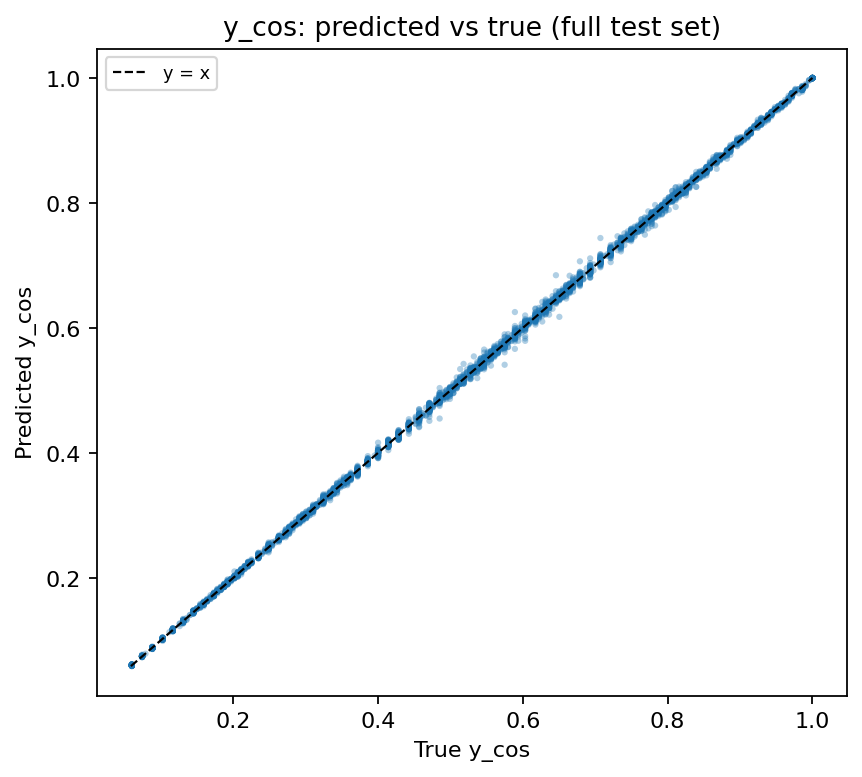
\includegraphics[width=\linewidth]{july16_rff_cos.png}
%   \caption{RFF}
% \end{subfigure}\hfill
% \begin{subfigure}[t]{0.32\textwidth}
%   \centering
%   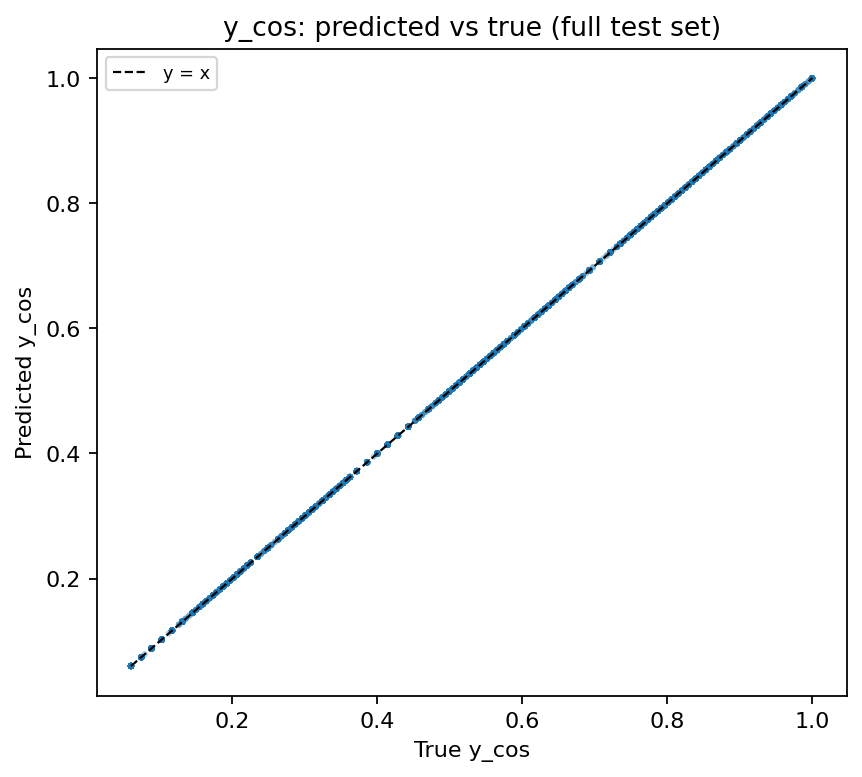
\includegraphics[width=\linewidth]{july16_orf_cos.png}
%   \caption{ORF}
% \end{subfigure}\hfill
% \begin{subfigure}[t]{0.32\textwidth}
%   \centering
%   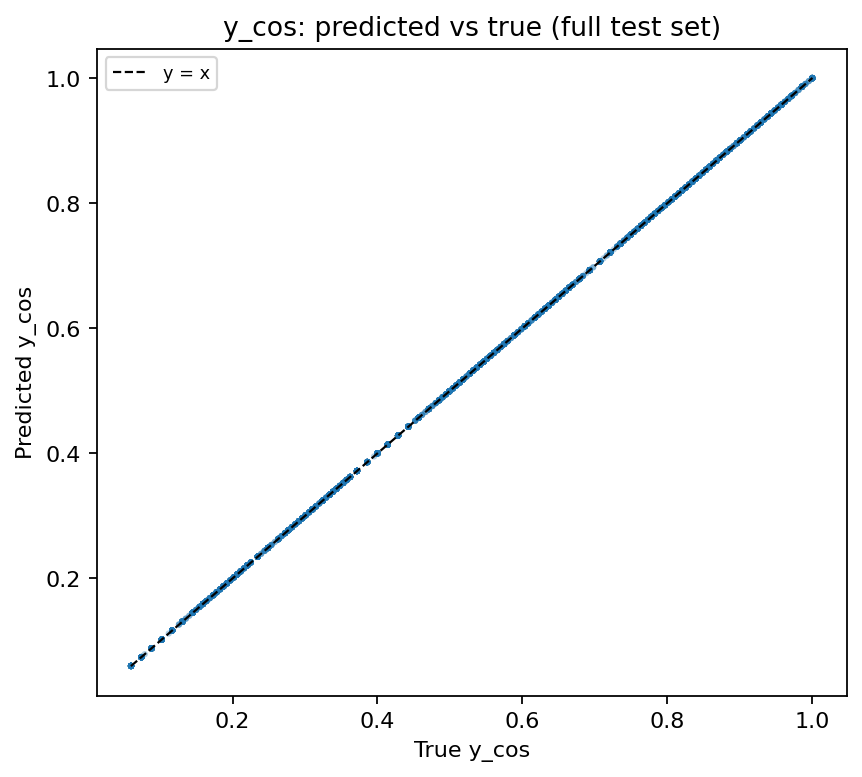
\includegraphics[width=\linewidth]{july16_sorf_cos.png}
%   \caption{SORF}
% \end{subfigure}
% \caption{July~16 $cos(i)$ true vs.\ prediction ($n=5000$, $\mathrm{lr}=0.01$)
% for RFF, ORF, and SORF.}
% \label{fig:july16-cos}
% \end{figure}

% A learning-rate sweep on ORF/SORF (Table~\ref{tab:lr-cost}, Figure~\ref{fig:lr-cost})
% identified $\mathrm{lr}=0.1$ as the best accuracy--cost balance; $\mathrm{lr}=1.0$
% trains much faster with only modest RRMSE degradation.

% \begin{table}[H]
% \centering
% \caption{July~16 learning-rate cost--performance (two QoI).}
% \label{tab:lr-cost}
% \scriptsize
% \begin{tabular}{llrrrr}
\toprule
Method & lr & Agg.\ RRMSE & Train time (s) & $cos(i)$ RRMSE & $grain\,size$ RRMSE \\
\midrule
ORF & 0.01 & 0.00506 & 4827 & 0.00068 & 0.00944 \\
ORF & 0.1 & 0.00489 & 2856 & 0.00069 & 0.00909 \\
ORF & 1 & 0.00647 & 173 & 0.00100 & 0.01194 \\
SORF & 0.01 & 0.00482 & 4834 & 0.00070 & 0.00895 \\
SORF & 0.1 & 0.00447 & 3373 & 0.00067 & 0.00827 \\
SORF & 1 & 0.00708 & 373 & 0.00097 & 0.01319 \\
RFF & 0.01 & 0.01312 & 669 & 0.01468 & 0.01156 \\
\bottomrule
\end{tabular}

% \end{table}

% \begin{figure}[H]
% \centering
% 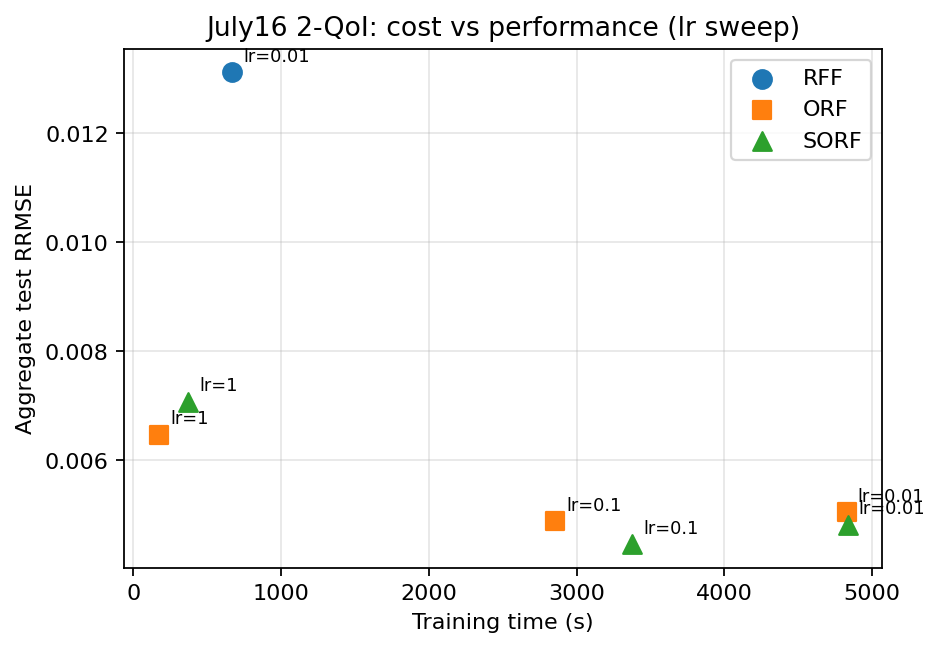
\includegraphics[width=0.72\textwidth]{lr_cost_performance.png}
% \caption{Aggregate test RRMSE vs.\ training time for the July~16 learning-rate sweep.}
% \label{fig:lr-cost}
% \end{figure}

% \FloatBarrier

% \subsection{Global eleven-QoI failure and pure-snow recovery}
% \label{sec:july23-29}

% On the unconstrained 11-QoI Sobol' design, linear radiance--QoI correlations were weak
% for most targets (Figure~\ref{fig:corr-11}).
% Independent SORF GPs ($D=400$) reached only aggregate RRMSE $0.596$
% (Table~\ref{tab:july23}); $cos(i)$ and $cwv$ were recoverable, while aerosols, dust,
% grain size, and algae were not (Figure~\ref{fig:july23-scatters}).

% \begin{figure}[H]
% \centering
% 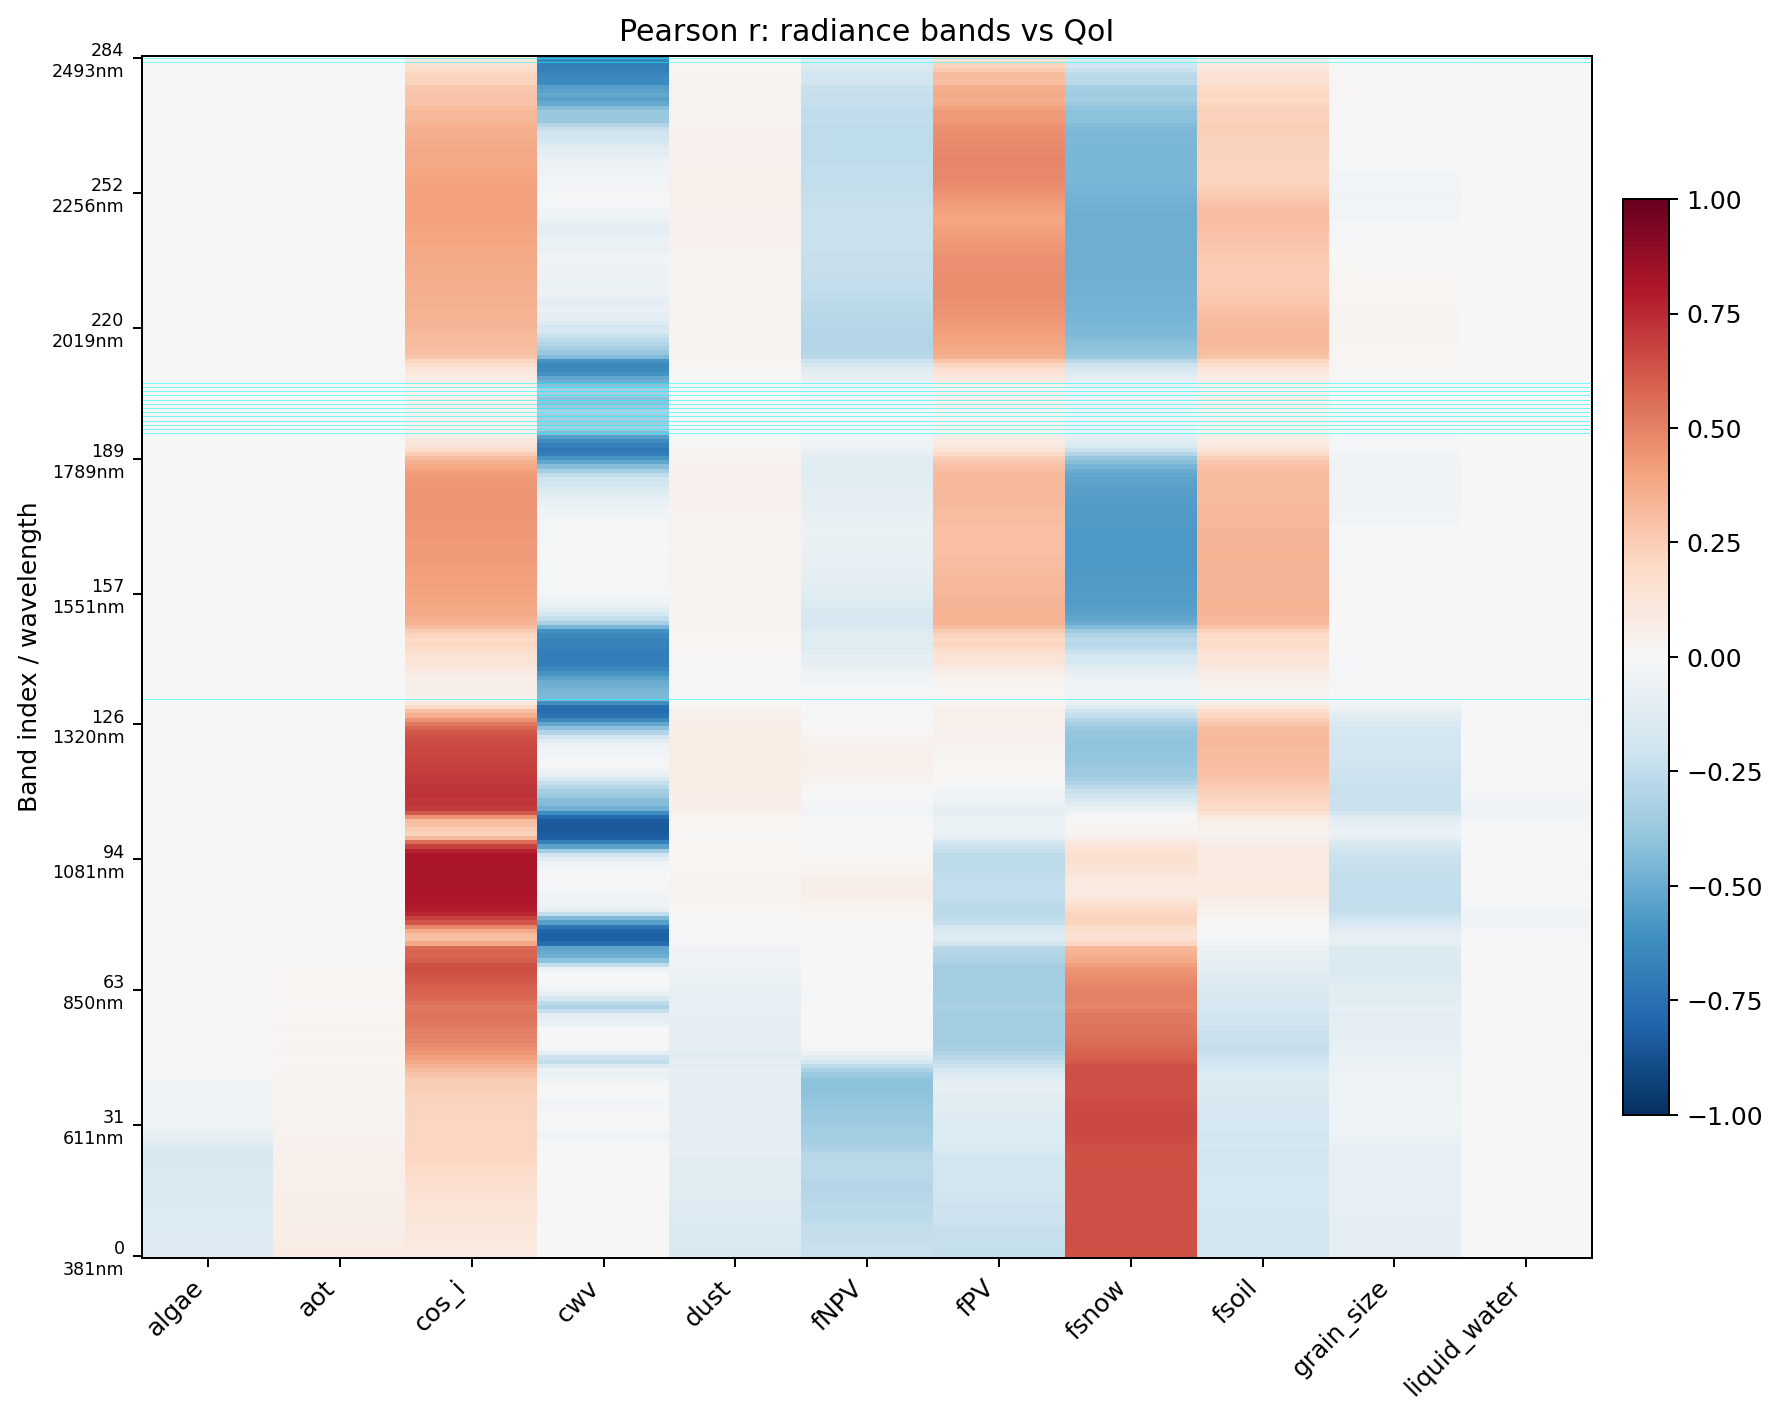
\includegraphics[width=0.88\textwidth]{corr_radiance_vs_qoi_11qoi.png}
% \caption{Radiance vs.\ QoI correlations on the full 11-QoI Sobol' dataset.}
% \label{fig:corr-11}
% \end{figure}

% \begin{table}[H]
% \centering
% \caption{July~23 full 11-QoI SORF results ($D=400$).}
% \label{tab:july23}
% \scriptsize
% \begin{tabular}{lrrrrr}
\toprule
QoI & RMSE & MAE & RRMSE & $R^2$ & NLPD \\
\midrule
algae & 1.207e+05 & 8.930e+04 & 0.6949 & 0.5171 & 13.126 \\
aot & 0.2674 & 0.2255 & 0.9656 & 0.0676 & 0.100 \\
cos\_i & 0.0123 & 0.0092 & 0.0452 & 0.9980 & -3.017 \\
cwv & 0.0344 & 0.0233 & 0.0239 & 0.9994 & -1.997 \\
dust & 978.5947 & 791.4438 & 0.8498 & 0.2778 & 8.308 \\
fNPV & 1.7743 & 1.4595 & 0.6132 & 0.6240 & 1.984 \\
fPV & 1.7878 & 1.4804 & 0.6157 & 0.6210 & 2.000 \\
fsnow & 1.6749 & 1.3812 & 0.5820 & 0.6613 & 1.935 \\
fsoil & 1.7679 & 1.4668 & 0.6080 & 0.6303 & 1.989 \\
grain\_size & 352.6900 & 286.9955 & 0.8328 & 0.3065 & 7.289 \\
liquid\_water & 5.2775 & 3.8969 & 0.7250 & 0.4744 & 3.087 \\
\midrule
\textbf{aggregate} & --- & --- & 0.5960 & --- & --- \\
\bottomrule
\end{tabular}

% \end{table}

% \begin{figure}[H]
% \centering
% \begin{subfigure}[t]{0.24\textwidth}
%   \centering
%   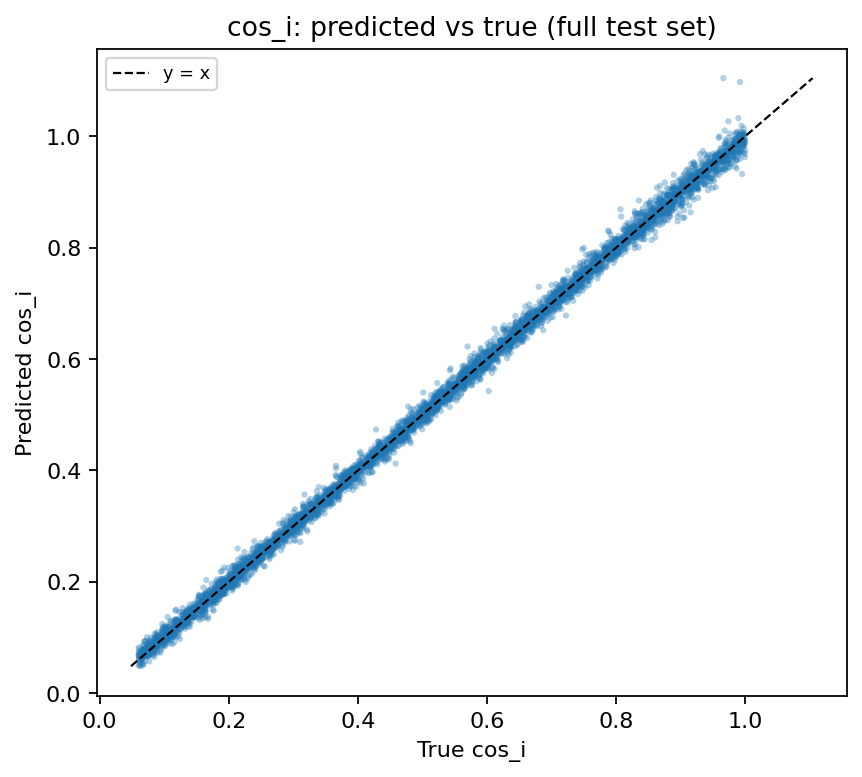
\includegraphics[width=\linewidth]{july23_cos.png}
%   \caption{$cos(i)$}
% \end{subfigure}\hfill
% \begin{subfigure}[t]{0.24\textwidth}
%   \centering
%   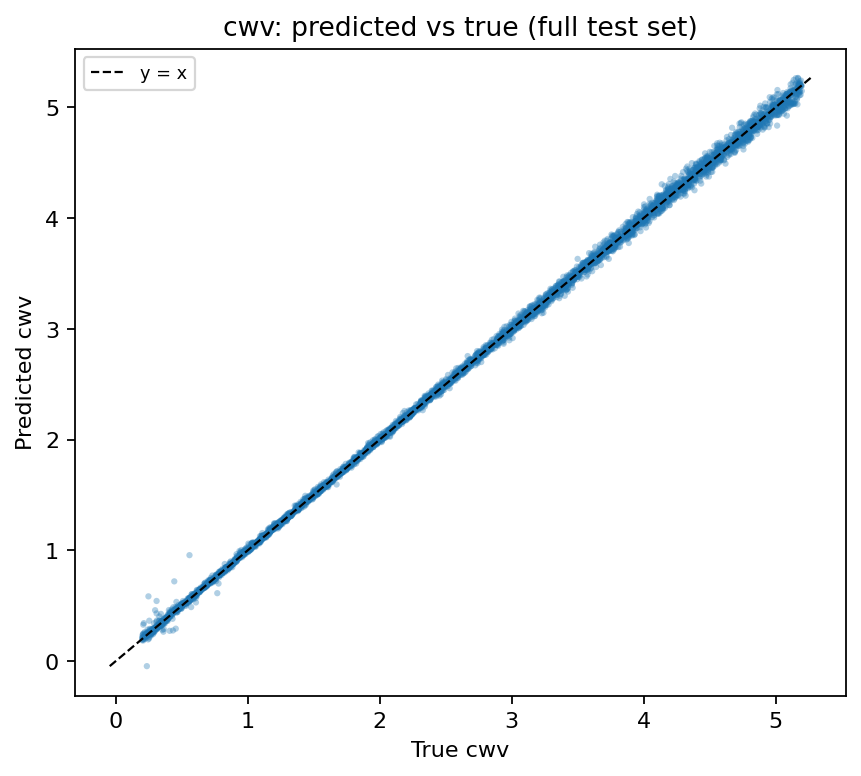
\includegraphics[width=\linewidth]{july23_cwv.png}
%   \caption{$cwv$}
% \end{subfigure}\hfill
% \begin{subfigure}[t]{0.24\textwidth}
%   \centering
%   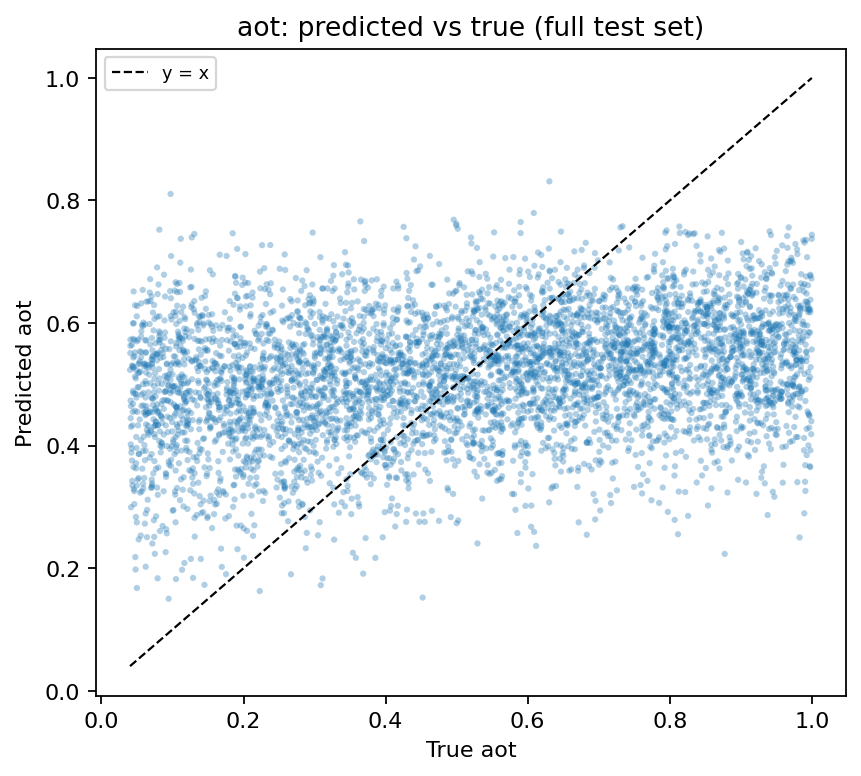
\includegraphics[width=\linewidth]{july23_aot.png}
%   \caption{$aot$}
% \end{subfigure}\hfill
% \begin{subfigure}[t]{0.24\textwidth}
%   \centering
%   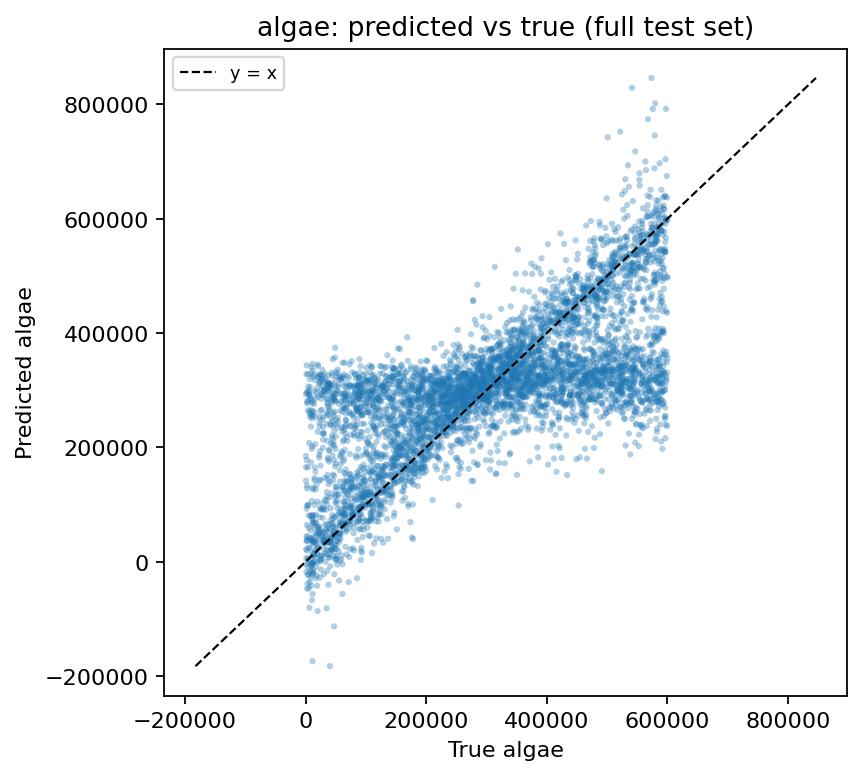
\includegraphics[width=\linewidth]{july23_algae.png}
%   \caption{$algae$}
% \end{subfigure}
% \caption{July~23 test scatters: recoverable ($cos(i)$, $cwv$) vs.\ hard ($aot$,
% $algae$) QoIs on the unconstrained design.}
% \label{fig:july23-scatters}
% \end{figure}

% Freezing the surface to pure snow strengthened radiance--QoI correlations
% (Figure~\ref{fig:corr-fsnow}).
% With $D=1600$, adjusted lengthscale initialization
% $\omega_i\sim\mathcal{N}(-4,1)$, and 2000 epochs, aggregate RRMSE fell to $0.0517$
% (Table~\ref{tab:july29-look})---roughly an order of magnitude better than the global
% design.
% Unbounded Gaussian predictives still placed a non-negligible fraction of means outside
% physical ranges (e.g., $\approx1.4\%$ of $aot$ predictions below the design floor
% $0.04$).

% \begin{figure}[H]
% \centering
% 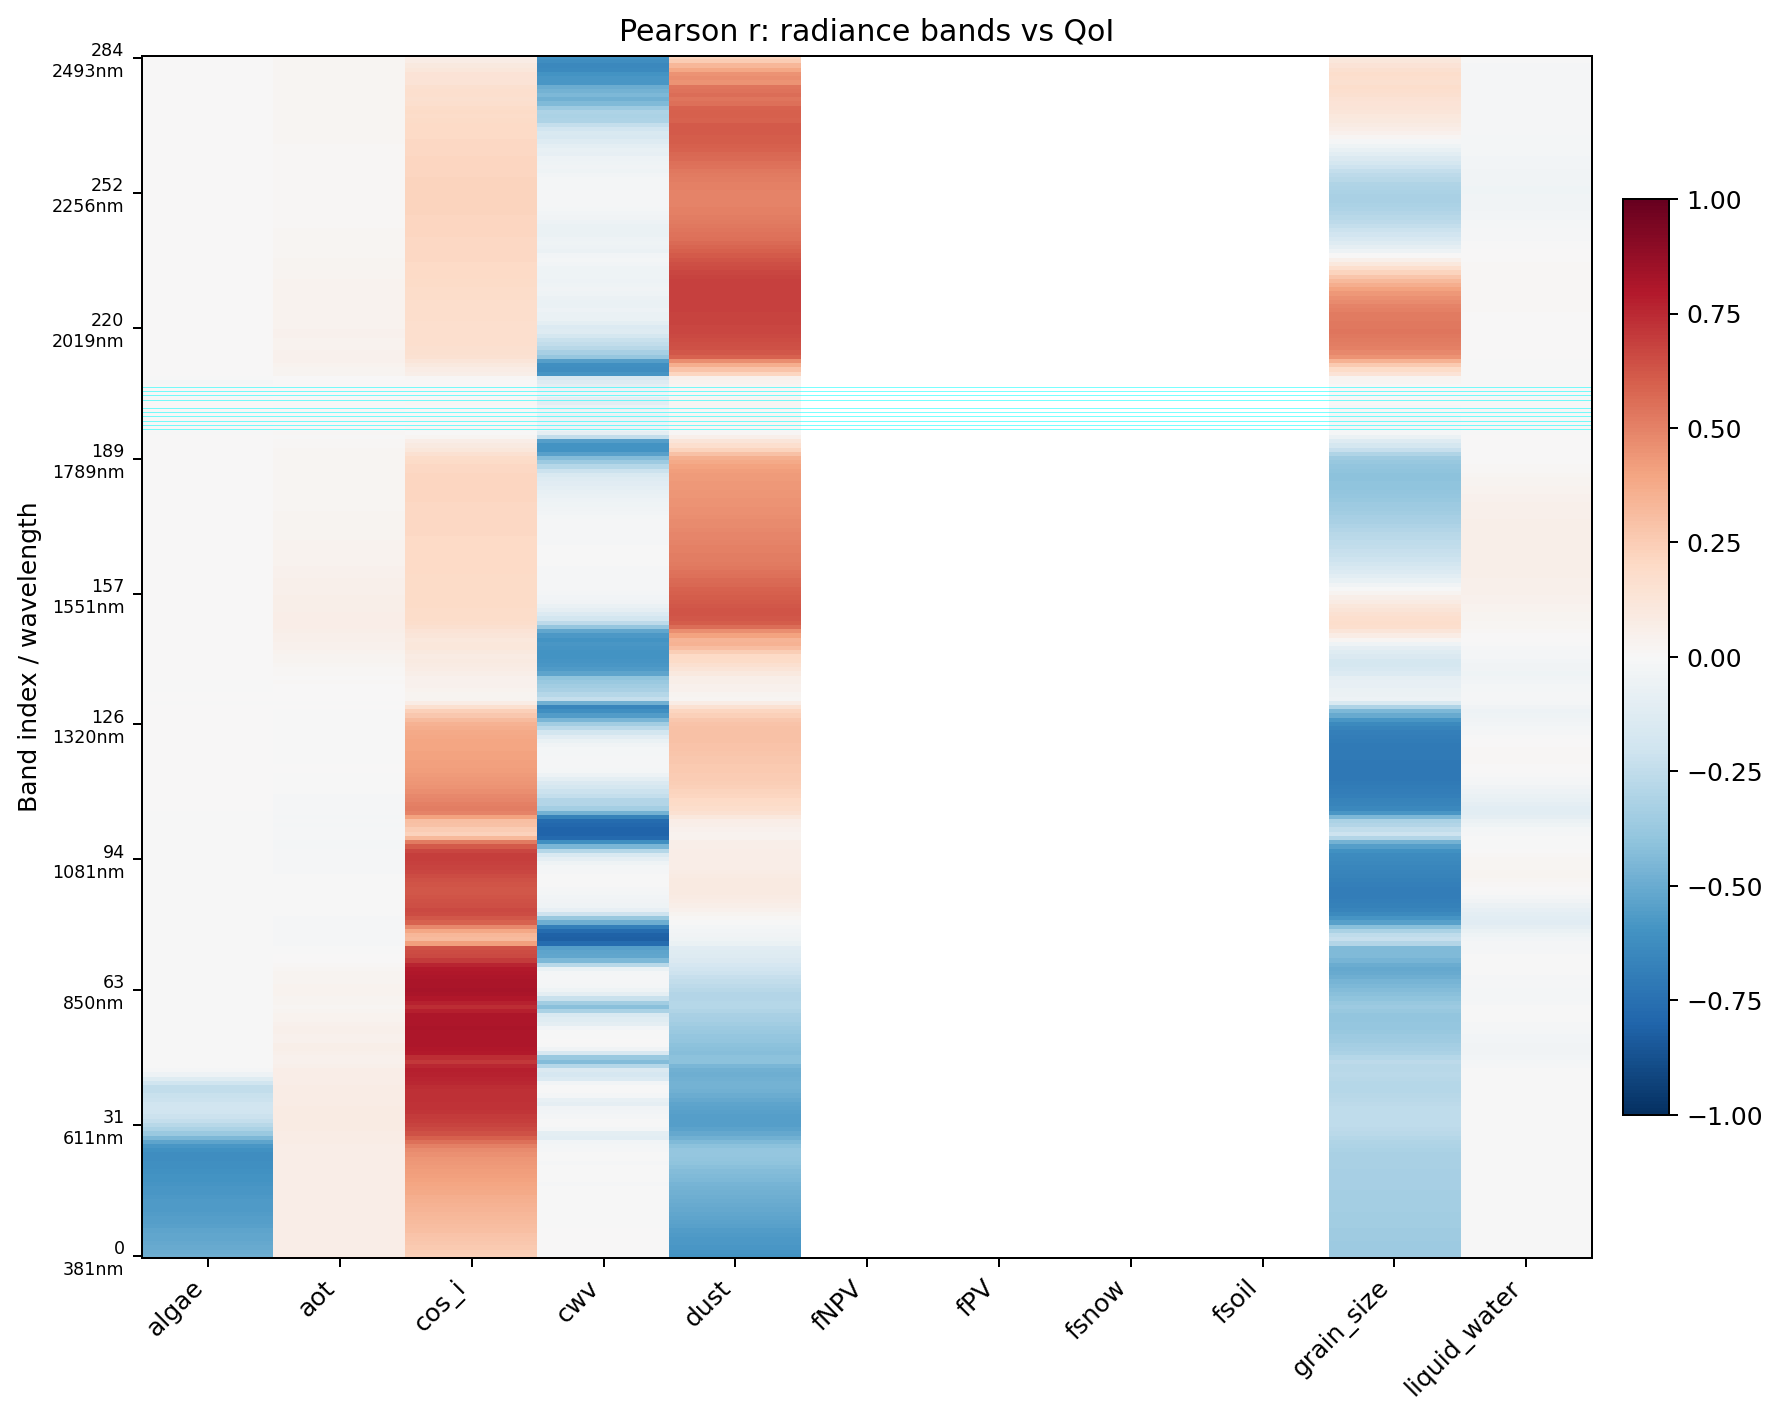
\includegraphics[width=0.88\textwidth]{corr_radiance_vs_qoi_fsnow_only.png}
% \caption{Radiance vs.\ QoI correlations for the fsnow-only (seven-QoI) dataset.}
% \label{fig:corr-fsnow}
% \end{figure}

% \begin{table}[H]
% \centering
% \caption{July~29 snow-only SORF ($D=1600$, adjusted lengthscale initialization).}
% \label{tab:july29-look}
% \scriptsize
% \begin{tabular}{lrrrrr}
\toprule
QoI & RMSE & MAE & RRMSE & $R^2$ & NLPD \\
\midrule
algae & 1.212e+04 & 5329.3018 & 0.0698 & 0.9951 & 10.415 \\
aot & 0.0260 & 0.0195 & 0.0939 & 0.9912 & -2.289 \\
cos\_i & 0.0211 & 0.0165 & 0.0779 & 0.9939 & -2.439 \\
cwv & 0.0431 & 0.0139 & 0.0300 & 0.9991 & -2.597 \\
dust & 59.8970 & 23.4219 & 0.0520 & 0.9973 & 4.897 \\
grain\_size & 6.3172 & 4.2157 & 0.0149 & 0.9998 & 3.193 \\
liquid\_water & 0.1685 & 0.1313 & 0.0231 & 0.9995 & -0.364 \\
\midrule
\textbf{aggregate} & --- & --- & 0.0517 & --- & --- \\
\bottomrule
\end{tabular}

% \end{table}

% Log/logit response warps and soft bound penalties did not adequately enforce physical
% support: unbounded Gaussian predictives can still place mass outside design ranges.

% \FloatBarrier

\subsection{Model Comparison on Flat $100\%$ Snow Covered Surface Simulated Data}
\label{sec:sept}

Tables~\ref{tab:sept-test-rrmse}--\ref{tab:sept-cost} summarize the
model comparison on the simulated data ($n_{\mathrm{train}}=10{,}000$, $n_{\mathrm{val}}=5{,}000$, $n_{\mathrm{test}}=25{,}000$).
On physics-based simulation test RRMSE, TabPFN achieves the best aggregate, closely followed
by a partitioned ensemble of PCA-GP. These are slightly misleading because algae and $aod$ are not recoverable in this regime. Every model had difficulty recovering these QoI, indicating irreducible problem hardness for those QoIs under the present design. 
Removing algae and aod from the aggregate score, some GP methods perform on par or better than the two aforementioned models.
Among random-feature and variational kernel methods, NI-SORF GP Mat\'ern-$3/2$ is strongest
overall and particularly accurate on $cos(i)$, grain size, and dust.

\begin{table}[H]
\centering
\caption{Physics-based simulation test RRMSE by QoI.}
\label{tab:sept-test-rrmse}
\scriptsize
\setlength{\tabcolsep}{4pt}
\begin{tabular}{lcccccccc}
\toprule
Model & cos i & grain & dust & algae & cwv & lwc & aot & Agg. \\
\midrule
NI-SVGP & 0.0047 & 0.0226 & 0.1525 & 1.0631 & 0.1033 & 0.1282 & 1.0000 & 0.3535 \\
PCA-SVGP & 0.0218 & 0.1922 & 0.1541 & 1.0317 & 0.0809 & 0.0273 & 0.9740 & 0.3546 \\
SORF & 0.0312 & 0.0602 & 0.3051 & 1.0418 & 0.1824 & 0.1966 & 1.0164 & 0.4048 \\
NI-SORF & 0.0013 & 0.0187 & 0.2937 & 1.0595 & 0.1215 & 0.1649 & 1.0455 & 0.3864 \\
NI-SORF Mat3/2 & 0.0004 & 0.0106 & 0.0240 & 1.0675 & 0.1300 & 0.1095 & 1.0993 & 0.3488 \\
NI-SORF-MTGP & 0.0339 & 0.0553 & 0.1027 & 1.0122 & 0.1342 & 0.2351 & 1.0261 & 0.3714 \\
TabPFN & 0.0035 & 0.0109 & 0.0314 & 0.9596 & 0.0624 & 0.0663 & 0.7866 & 0.2744 \\
PCA-GP & 0.0209 & 0.0530 & 0.0140 & 0.9754 & 0.0753 & 0.0185 & 0.7864 & 0.2776 \\
\bottomrule
\end{tabular}
\end{table}

Test NIS scores (Table~\ref{tab:sept-test-nis}) show a similar pattern where TabPFN and
PCA-GP lead on several QoIs, while NI-SORF Mat\'ern-$3/2$ remains competitive among
the set of other GP-based emulators.

\begin{table}[H]
\centering
\caption{Physics-based simulation test NIS by QoI.}
\label{tab:sept-test-nis}
\scriptsize
\setlength{\tabcolsep}{4pt}
\begin{tabular}{lccccccc}
\toprule
Model & cos i & grain & dust & algae & cwv & lwc & aot \\
\midrule
NI-SVGP & 0.0696 & 0.1246 & 1.6102 & 5.0372 & 0.6375 & 0.7567 & 3.9788 \\
PCA-SVGP & 0.1113 & 1.2284 & 1.3542 & 4.9206 & 0.5274 & 0.1820 & 3.8859 \\
SORF & 0.1109 & 0.2693 & 2.3211 & 4.8810 & 0.9830 & 0.9788 & 3.9670 \\
NI-SORF & 0.0140 & 0.0755 & 1.9942 & 5.6052 & 0.6623 & 0.7402 & 4.3222 \\
NI-SORF Mat3/2 & 0.0132 & 0.0414 & 0.0936 & 5.4553 & 0.6970 & 0.5643 & 5.5511 \\
NI-SORF-MTGP & 0.2096 & 0.3071 & 0.5816 & 10.1830 & 0.7658 & 1.4989 & 4.0989 \\
TabPFN & 0.0328 & 0.0524 & 0.1487 & 3.1207 & 0.2691 & 0.4639 & 3.1063 \\
PCA-GP & 0.1104 & 0.2887 & 0.0720 & 3.9419 & 0.4637 & 0.0925 & 3.7022 \\
\bottomrule
\end{tabular}
\end{table}

On the ASD field spectra, RRMSE (Table~\ref{tab:sept-asd-rrmse}) is elevated for every method
and RRMSE is close to or exceeds one for most QoI.
Even TabPFN, strongest on physics-based simulation test, degrades to aggregate ASD RRMSE $2.48$.
Per-QoI ASD coverage grids (Figure~\ref{fig:asd-coverage}) further indicate
miscalibration on field scenes. The predictive intervals that look reasonable on simulator
test data do not reliably cover ASD-derived labels. PCA-GP is a clear example of this where it performs best on dust and lwc in the simulation data, but is not the best performing on the ASD field spectra.

\begin{table}[H]
\centering
\caption{Sept.\ ASD transfer RRMSE by QoI (FieldSpec-4 / DISORT labels).}
\label{tab:sept-asd-rrmse}
\scriptsize
\setlength{\tabcolsep}{4pt}
\begin{tabular}{lcccccccc}
\toprule
Model & cos i & grain & dust & algae & cwv & lwc & aot & Agg. \\
\midrule
NI-SVGP & 0.1753 & 0.3874 & 0.9564 & 4.2017 & 1.5451 & 0.3416 & 1.6623 & 1.3243 \\
PCA-SVGP & 0.6367 & 0.8783 & 1.2279 & 6.5291 & 1.4734 & 0.3498 & 1.7723 & 1.8382 \\
SORF & 1.1543 & 1.1696 & 1.1887 & 3.0040 & 1.4685 & 1.5556 & 1.5624 & 1.5861 \\
NI-SORF & 0.1557 & 0.5594 & 0.9904 & 13.1585 & 1.4129 & 2.1599 & 1.9661 & 2.9147 \\
NI-SORF Mat3/2 & 0.0381 & 0.4377 & 2.9278 & 8.2718 & 1.1877 & 0.9537 & 2.7140 & 2.3615 \\
NI-SORF-MTGP & 1.1308 & 0.4851 & 0.7648 & 26.9851 & 1.1298 & 1.5880 & 3.0057 & 5.0128 \\
TabPFN & 0.2686 & 0.4571 & 0.7507 & 11.8454 & 1.5494 & 1.2821 & 1.2089 & 2.4803 \\
PCA-GP & 0.7646 & 0.4181 & 2.9761 & 15.0293 & 1.4609 & 0.4768 & 7.2055 & 4.0473 \\
\bottomrule
\end{tabular}
\end{table}

\begin{figure}[H]
\centering
\begin{subfigure}[t]{0.80\textwidth}
  \centering
  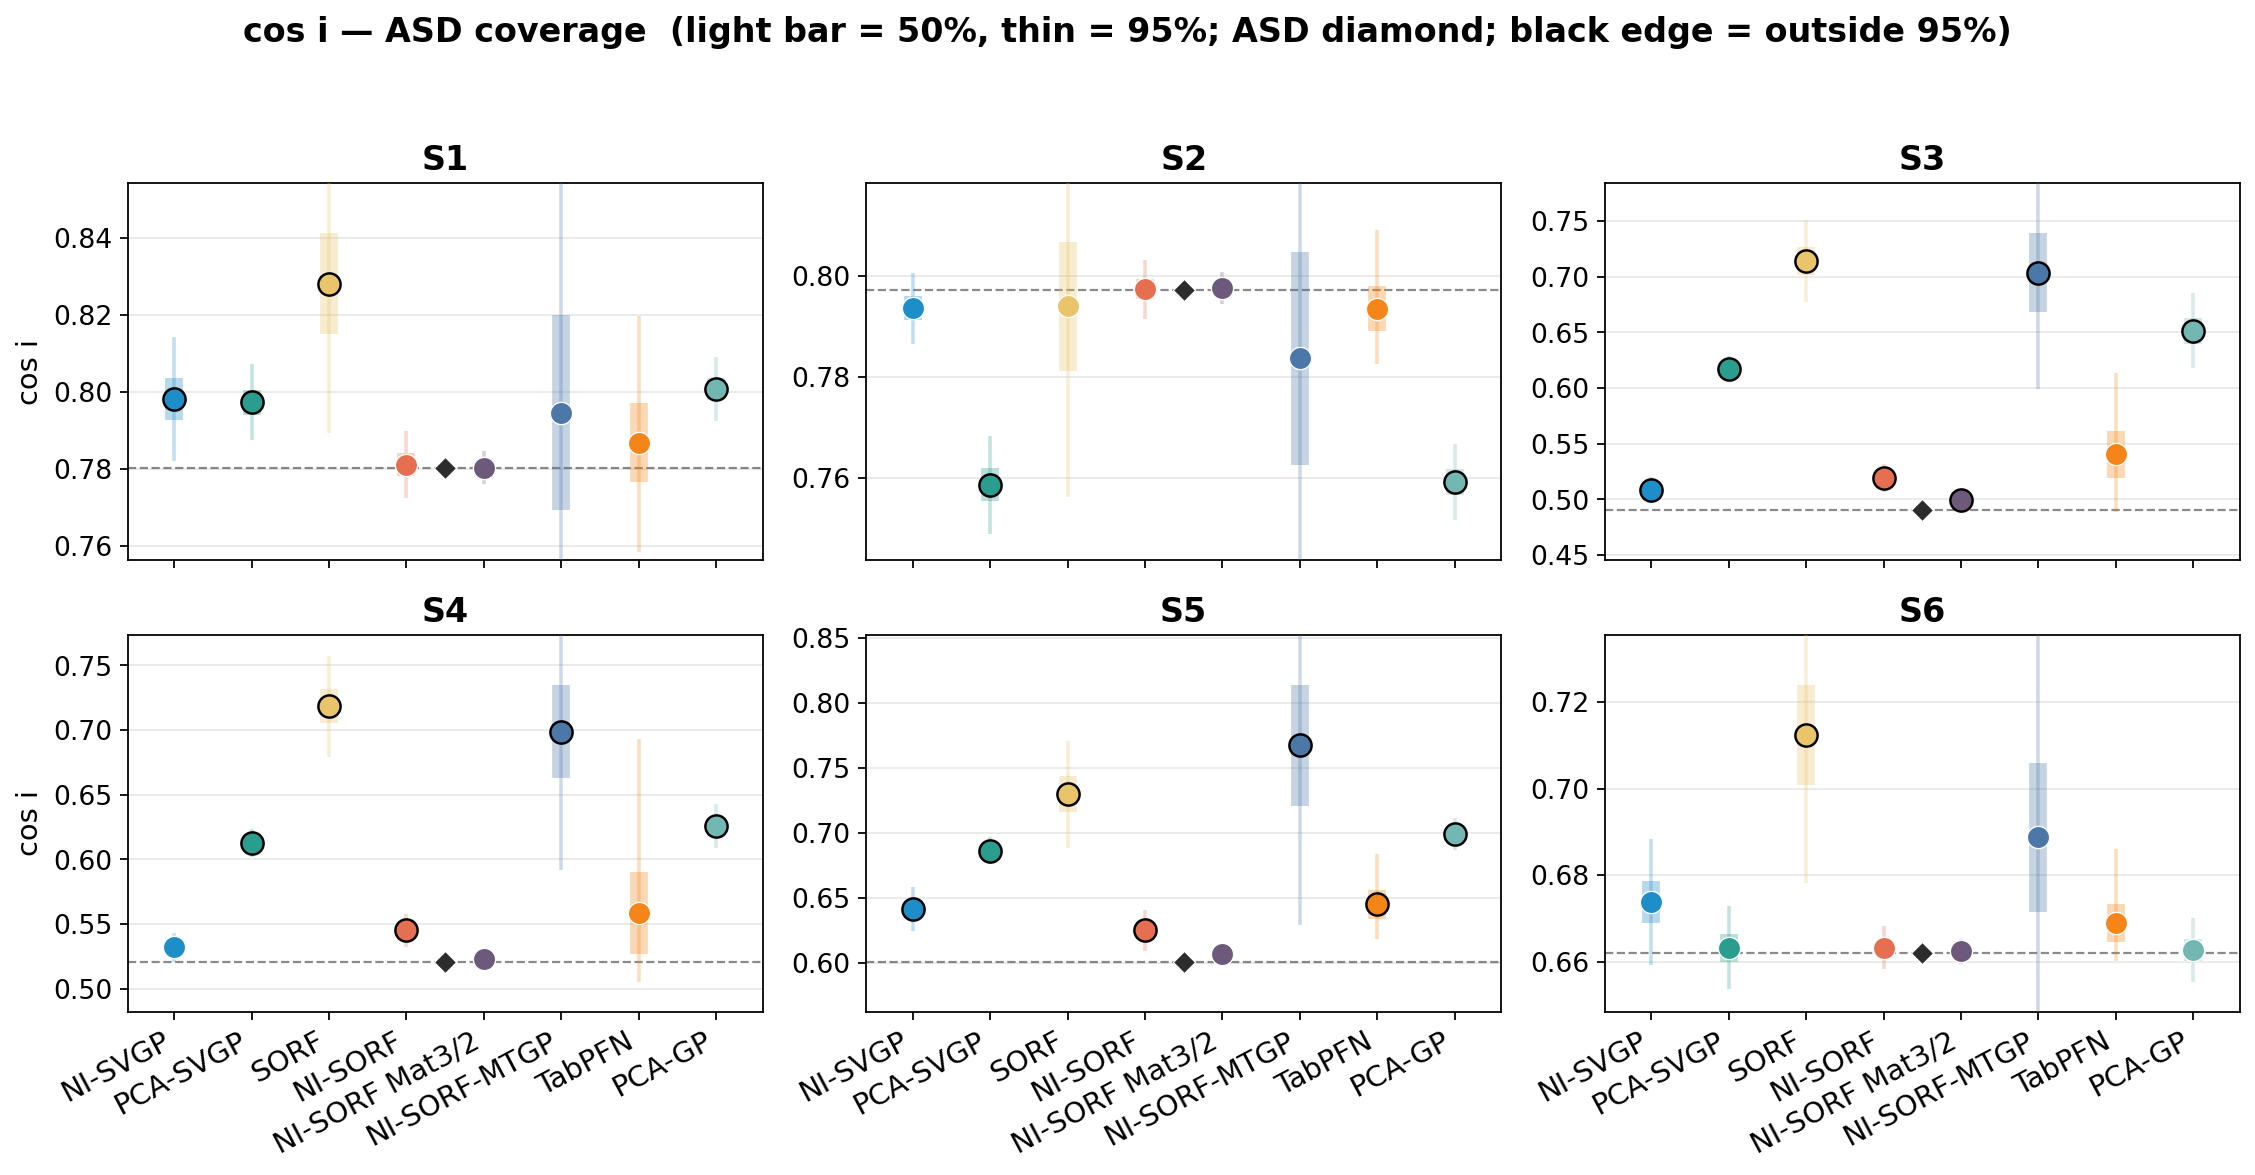
\includegraphics[width=\linewidth]{asd_coverage_cos_i.png}
  \caption{$cos(i)$}
\end{subfigure}\vfill
\begin{subfigure}[t]{0.8\textwidth}
  \centering
  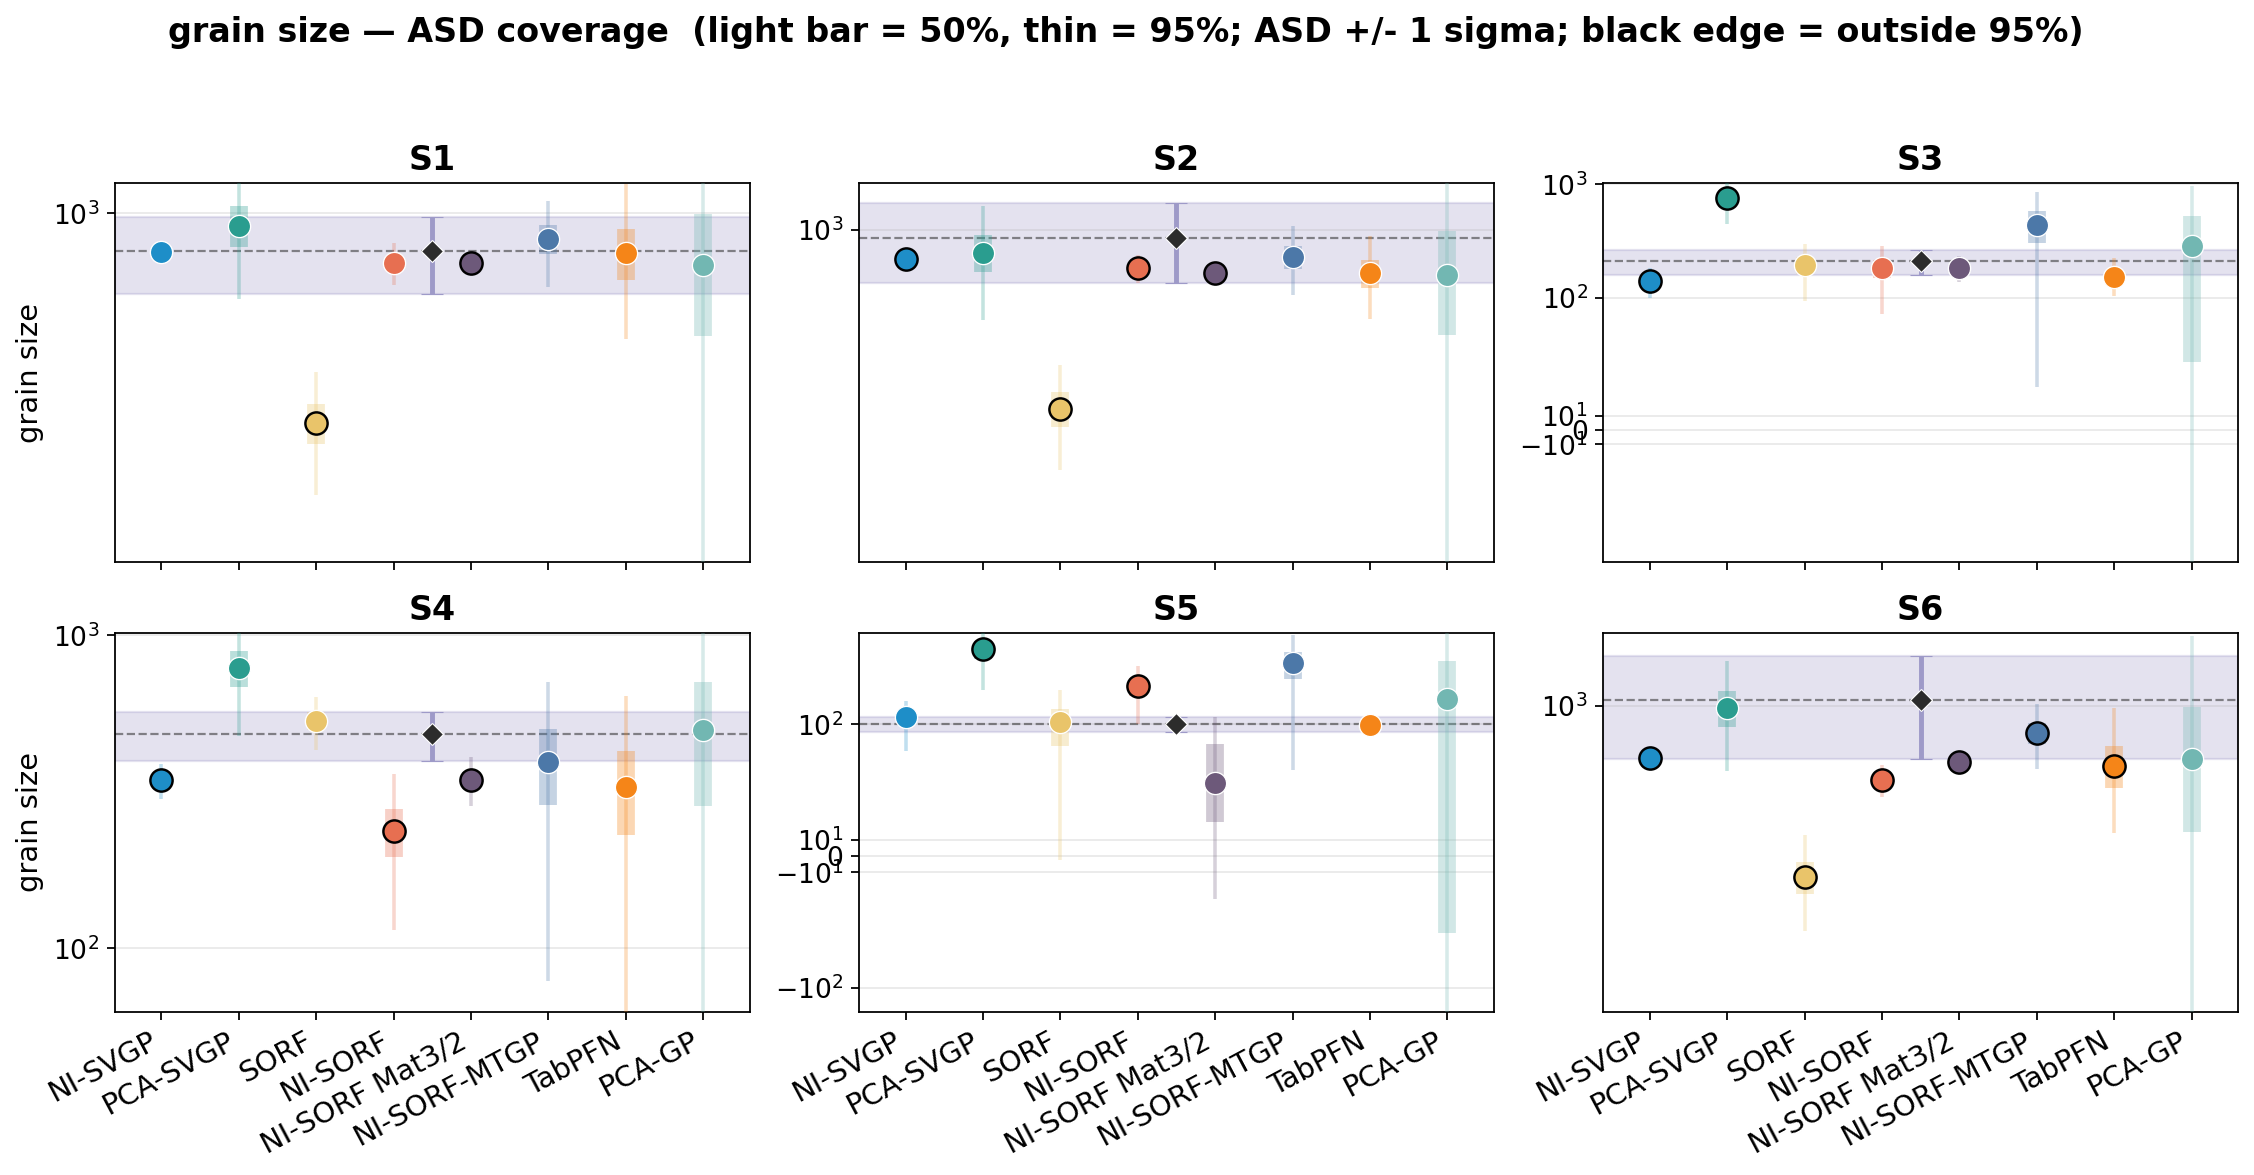
\includegraphics[width=\linewidth]{asd_coverage_grain_size.png}
  \caption{grain size}
\end{subfigure}\vfill
\begin{subfigure}[t]{0.8\textwidth}
  \centering
  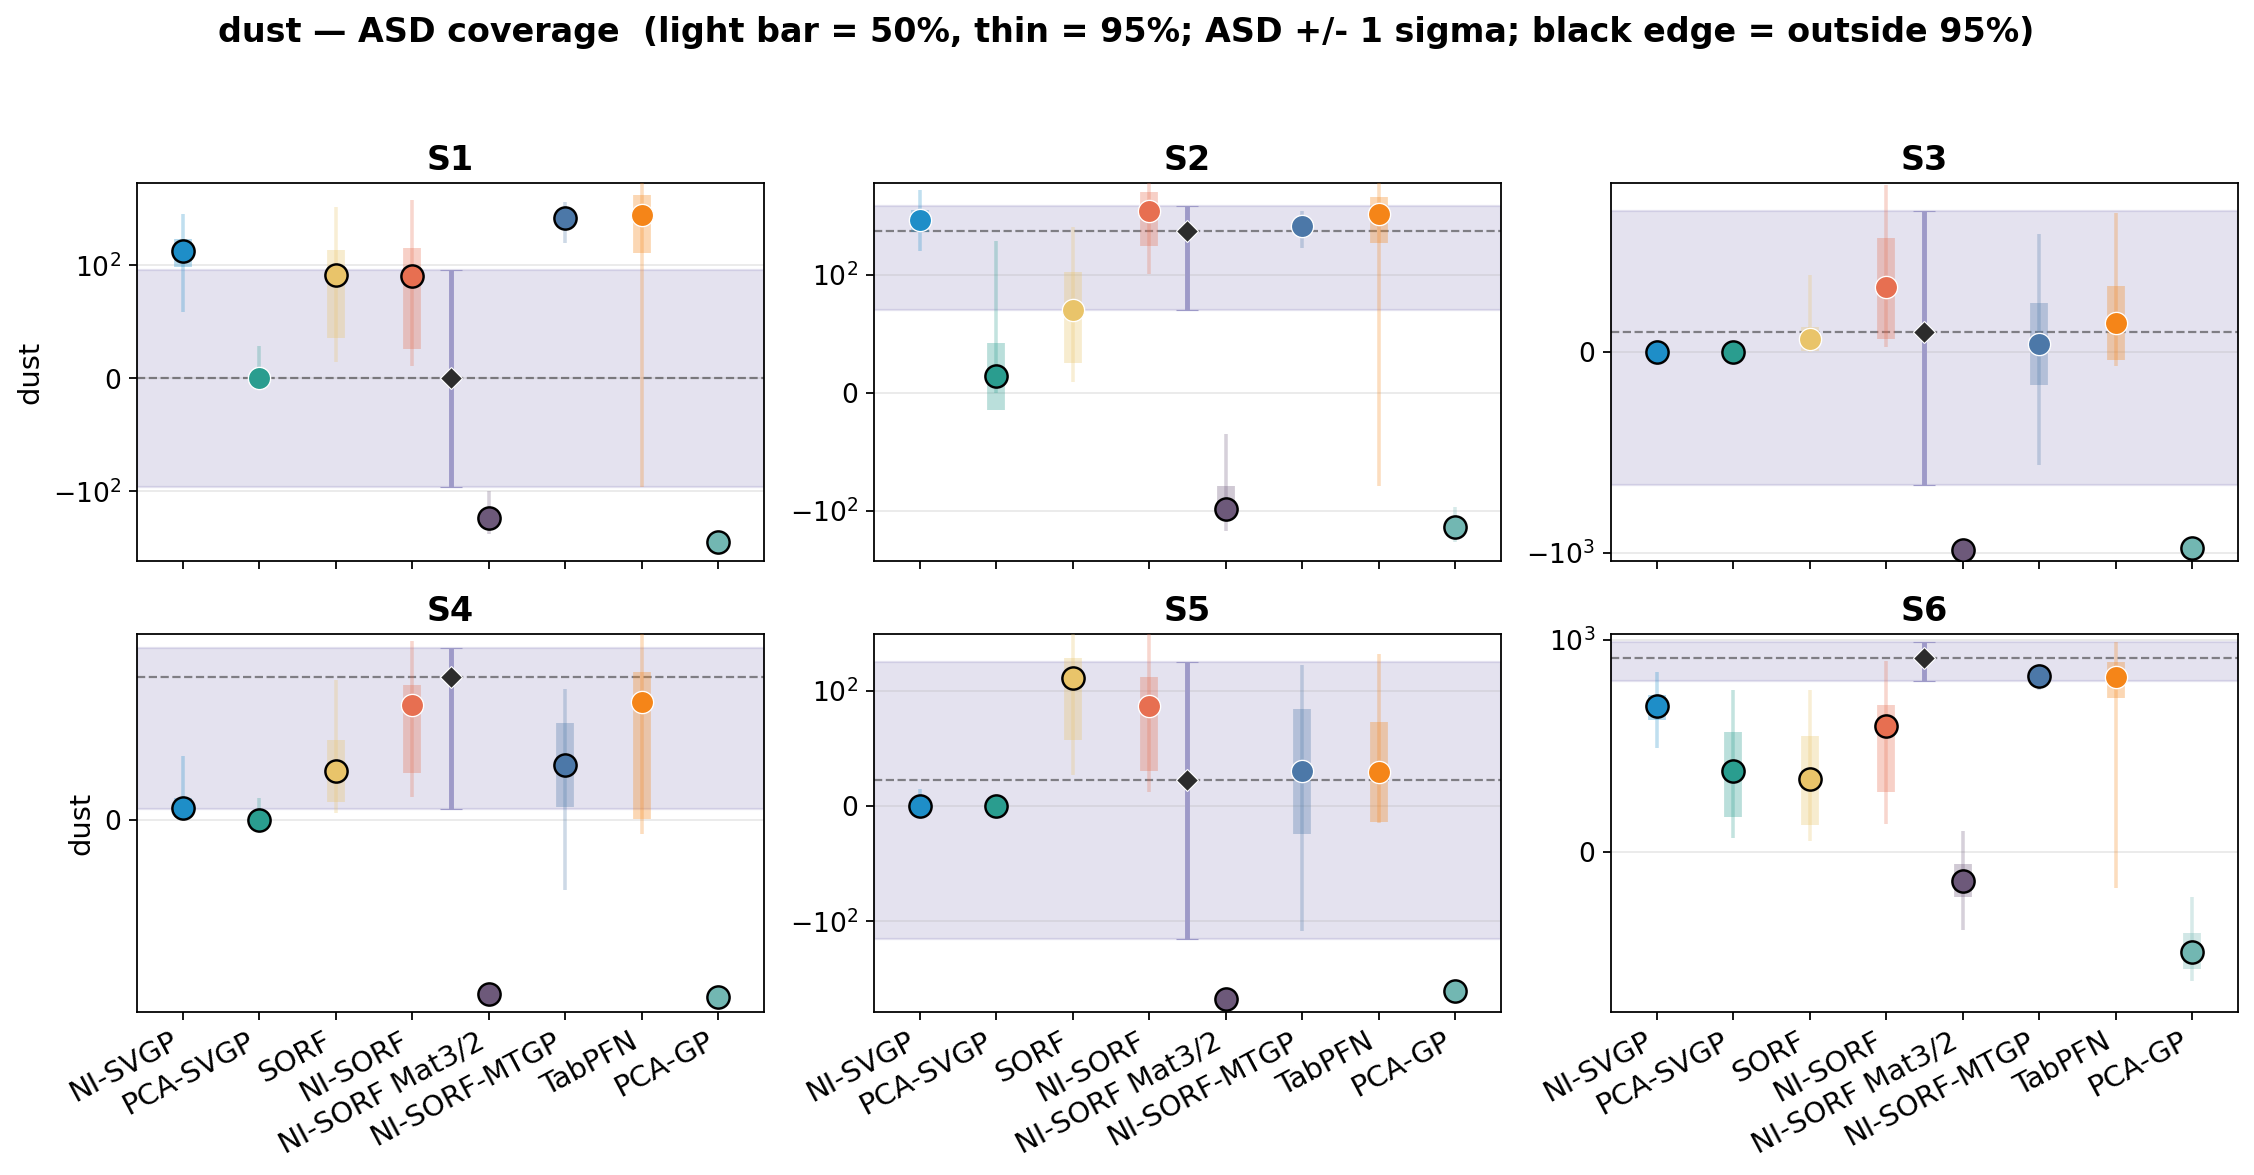
\includegraphics[width=\linewidth]{asd_coverage_dust.png}
  \caption{dust}
\end{subfigure}
\caption{ASD predictive coverage by model for three QoIs.
Elevated RRMSE coincides with miscalibrated coverage on field scenes.}
\label{fig:asd-coverage}
\end{figure}

Training and inference costs with each model architecture are shown in Table~\ref{tab:sept-cost}.
SVGP variants finish training in under an hour and predict on all QoI in about one second.
SORF-family and MTGP models with the noisy-input term require multi-hour training and minutes of inference.
TabPFN fits in tens of seconds but requires hours to predict on the test set, which does not fit the problem's needs of needing to keep inference cost low.

\begin{table}[H]
\centering
\caption{Training and inference wall-clock cost}
\label{tab:sept-cost}
\scriptsize
\begin{tabular}{llrrr}
\toprule
Model & Architecture & Epochs & Train & Infer \\
\midrule
NI-SVGP & SVGP+NIGP, M=512, indep. & 300 & 33.1 min & 1.13 s \\
PCA-SVGP & PCA$\to$SVGP, M=512, P/QoI & 300 & 44.0 min & 0.87 s \\
SORF & SORF-RFF GP, D=2000, RBF & 700 & 2.40 h & 19.30 s \\
NI-SORF & SORF-RFF+NIGP, D=2000, RBF & 700 & 2.13 h & 1.5 min \\
NI-SORF Mat3/2 & SORF-RFF+NIGP, D=2400, Mat3/2 & 1000 & 3.55 h & 2.1 min \\
NI-SORF-MTGP & Joint SORF-MTGP+NIGP, D=1600, r=1 & 200 & 3.44 h & 15.5 min \\
TabPFN & TabPFNRegressor & --- & 34.26 s & 7.33 h \\
PCA-GP & PCA$\to$exact GP, LBFGS CPU, part=2000, top-5 & 1 & 5.73 h & 32.34 s \\
\bottomrule
\end{tabular}

\end{table}

\subsection{Spectral Neighbors}
\label{sec:neighbor}

We performed diagnostics for nearest spectral neighbors (Figure~\ref{fig:asd-neighbors}) and ASD nearest-neighbor counts by
dataset (Figure~\ref{fig:asd-nn}) to help explain the transfer gap between the simulations and the field spectra. The other datasets examined were flat surfaces with $90-100\%$ snow coverage and surfaces at varying slopes with $90-100\%$ snow coverage. Field spectra often lie
far from the physics-based simulation training cloud in spectral space, so emulator interpolation
becomes extrapolation.
Grain-size paired scatter plots against the other QoIs (Figure~\ref{fig:asd-grain-pairs}) further show how ASD labels sit relative to the simulator cloud in joint QoI space.

\begin{figure}[H]
\centering
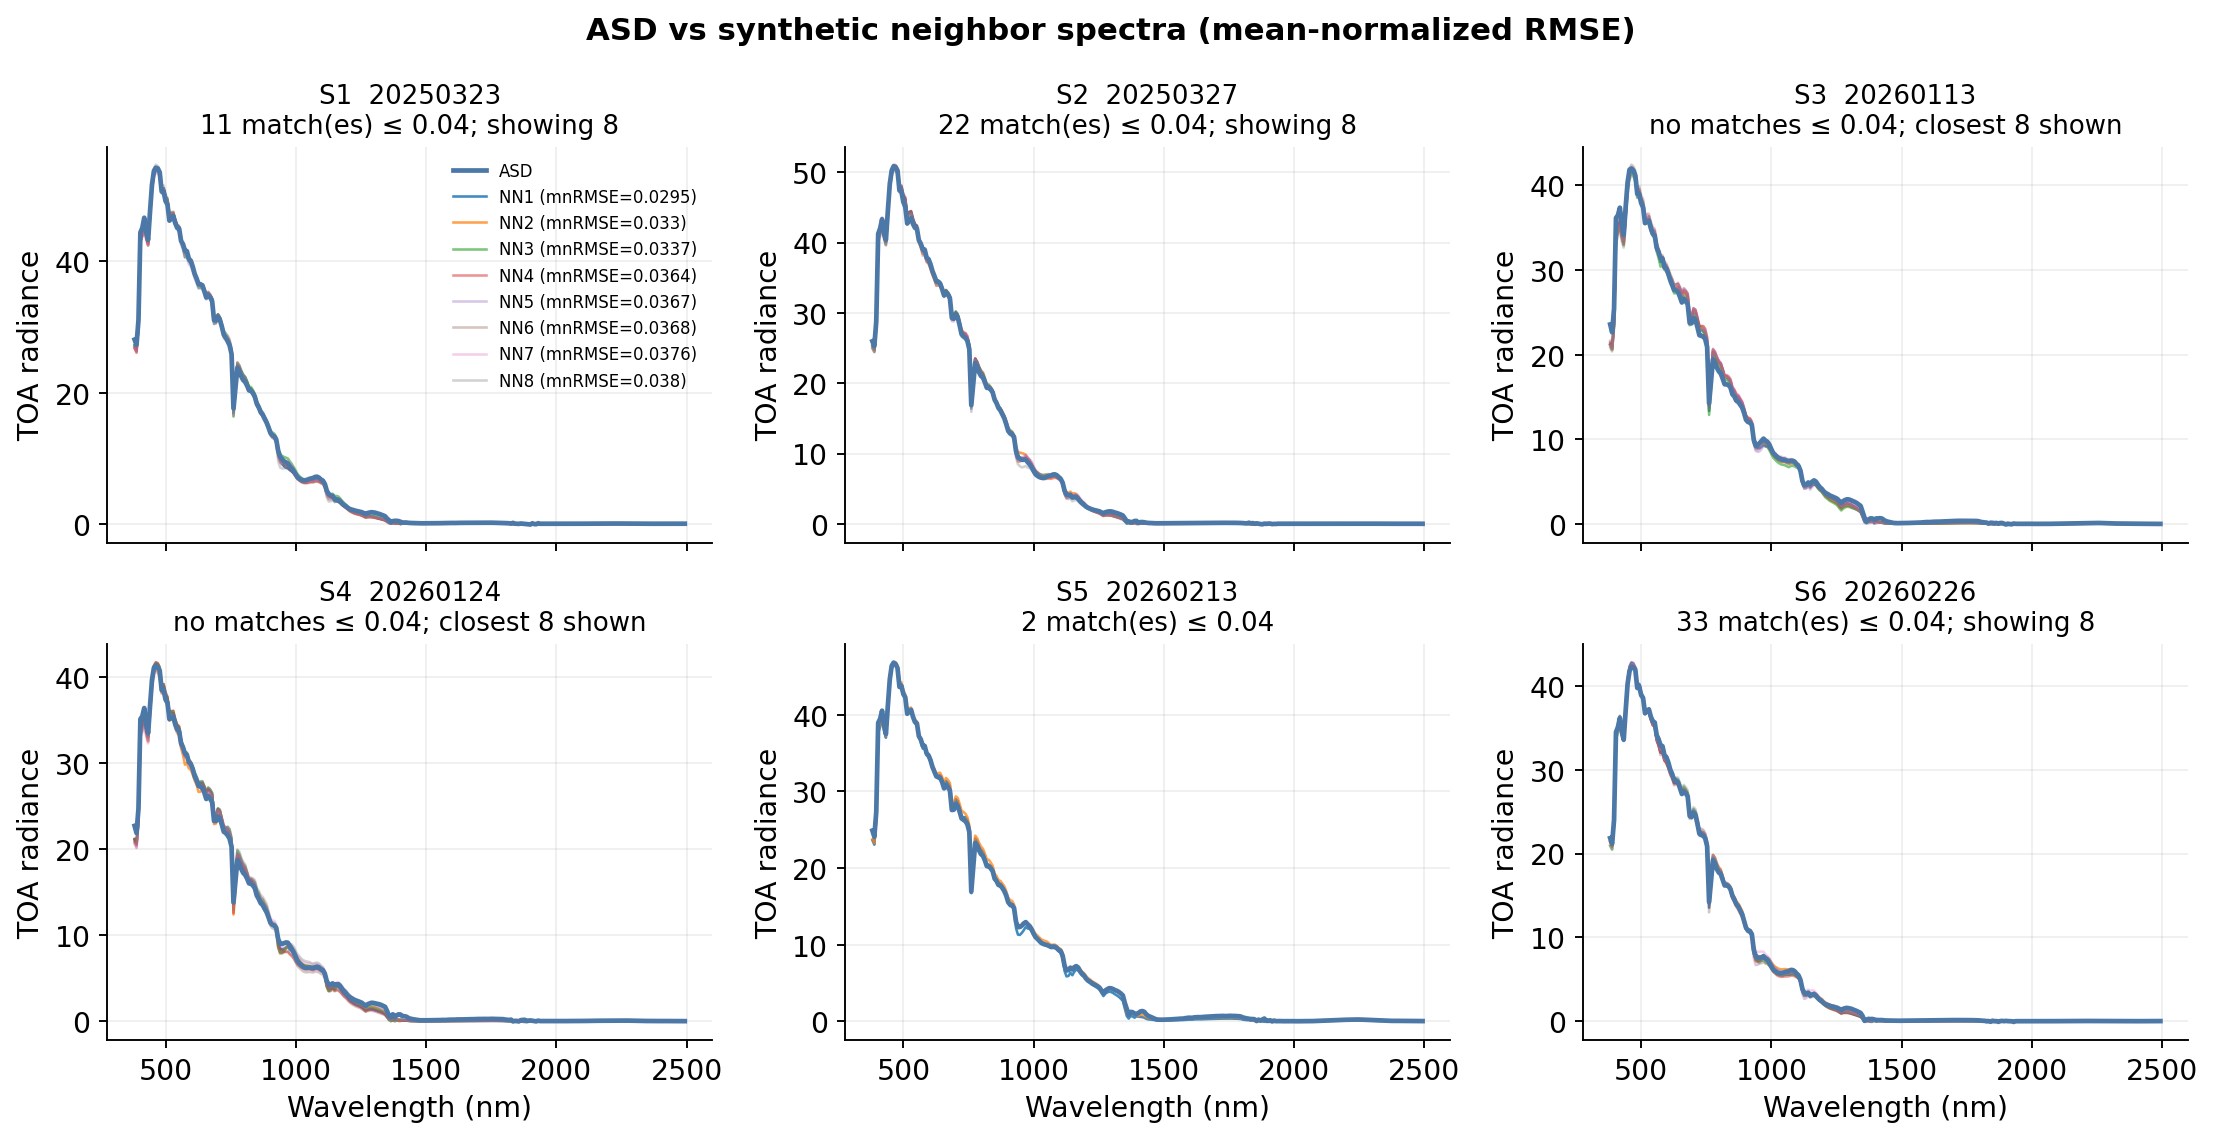
\includegraphics[width=0.85\textwidth]{spectra_neighbors_mnRMSE.png}
\caption{ASD spectra neighbors ranked by mean normalized RMSE (NI-SORF Mat\'ern-$3/2$
validation folder).}
\label{fig:asd-neighbors}
\end{figure}

\begin{figure}[H]
\centering
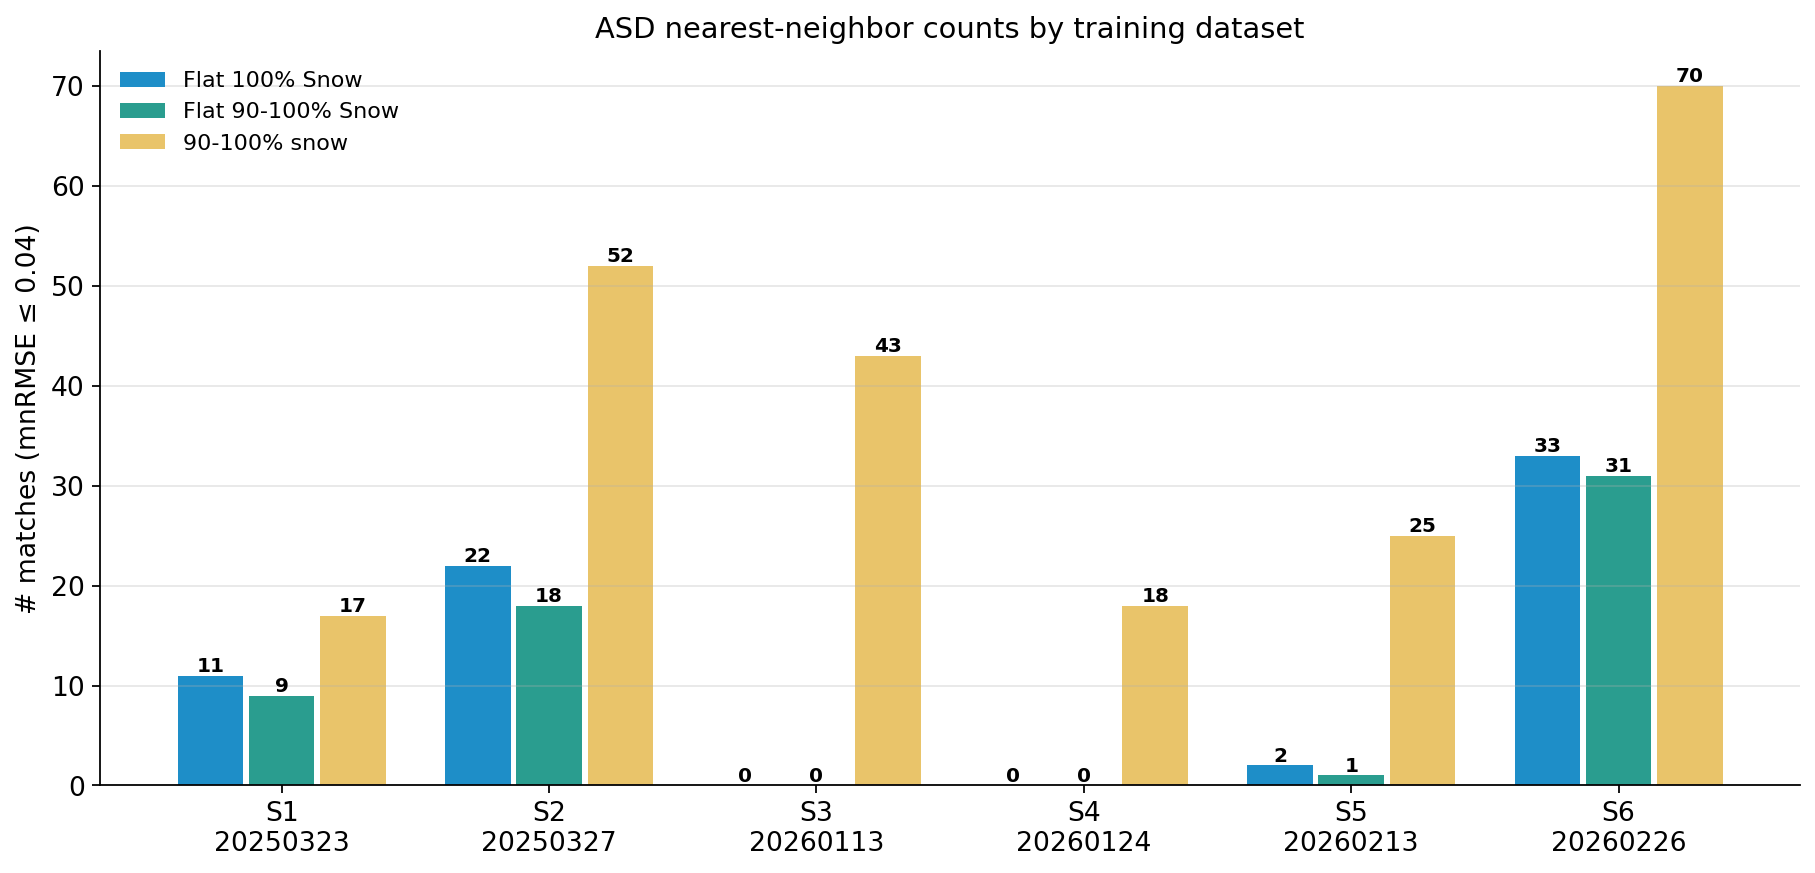
\includegraphics[width=0.75\textwidth]{asd_nn_counts_by_dataset.png}
\caption{ASD nearest-neighbor counts by dataset, illustrating limited spectral overlap
with physics-based simulation TOA training draws.}
\label{fig:asd-nn}
\end{figure}

\begin{figure}[H]
\centering
\begin{subfigure}[t]{0.32\textwidth}
  \centering
  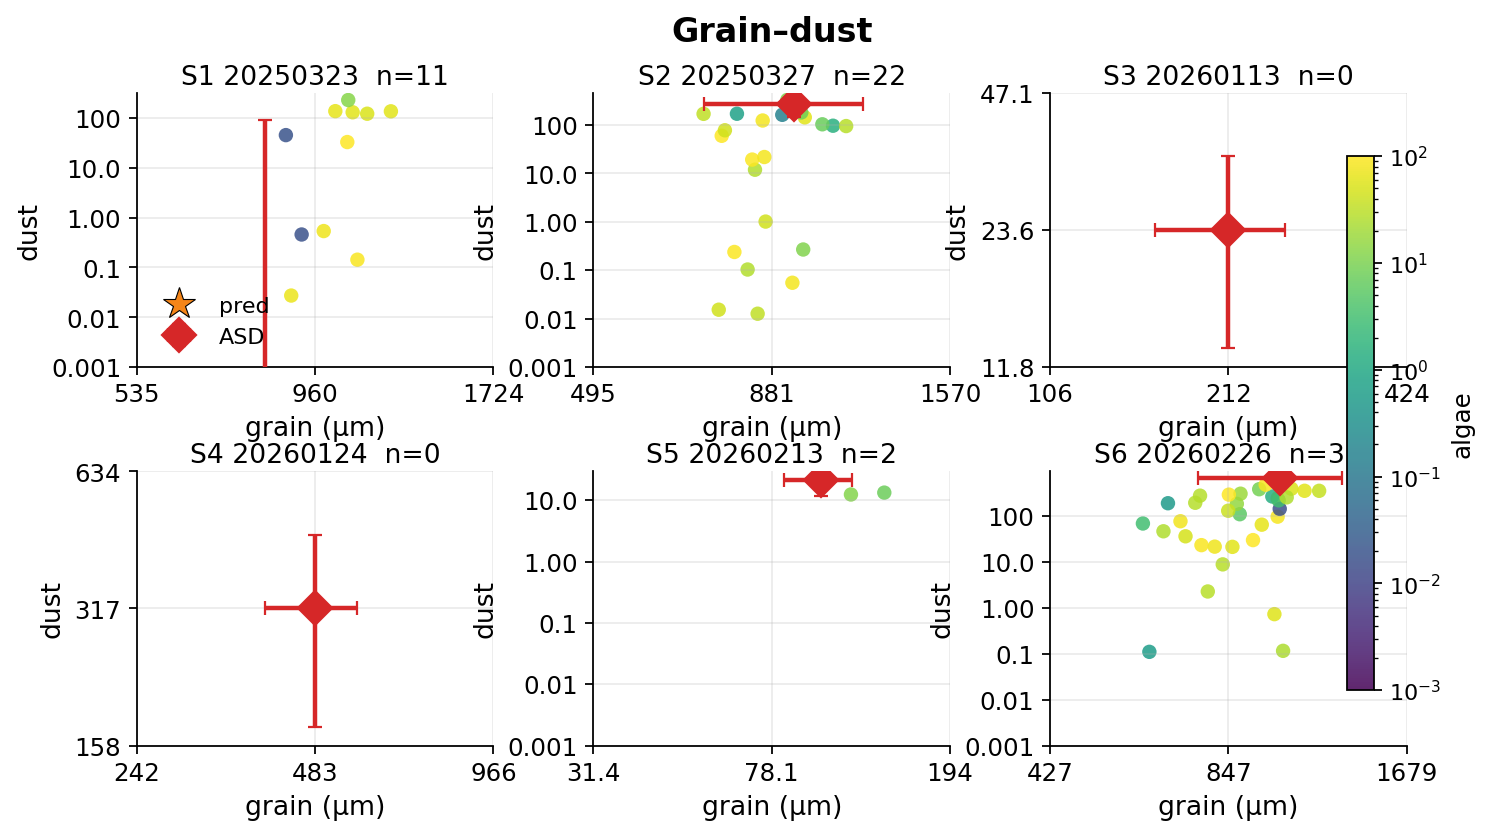
\includegraphics[width=\linewidth]{grain_dust.png}
  \caption{grain vs.\ dust}
\end{subfigure}\hfill
\begin{subfigure}[t]{0.32\textwidth}
  \centering
  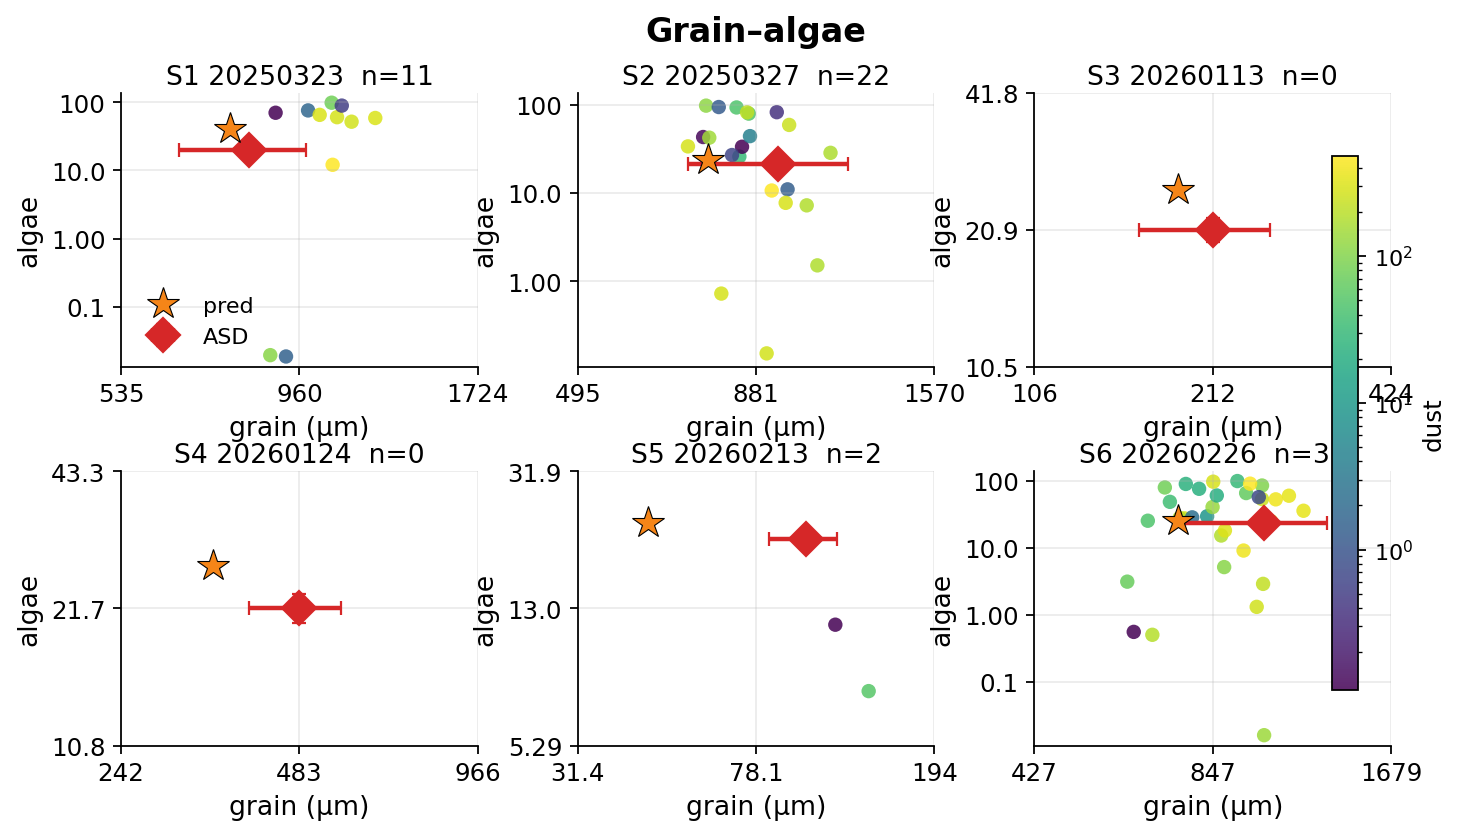
\includegraphics[width=\linewidth]{grain_algae.png}
  \caption{grain vs.\ algae}
\end{subfigure}\hfill
\begin{subfigure}[t]{0.32\textwidth}
  \centering
  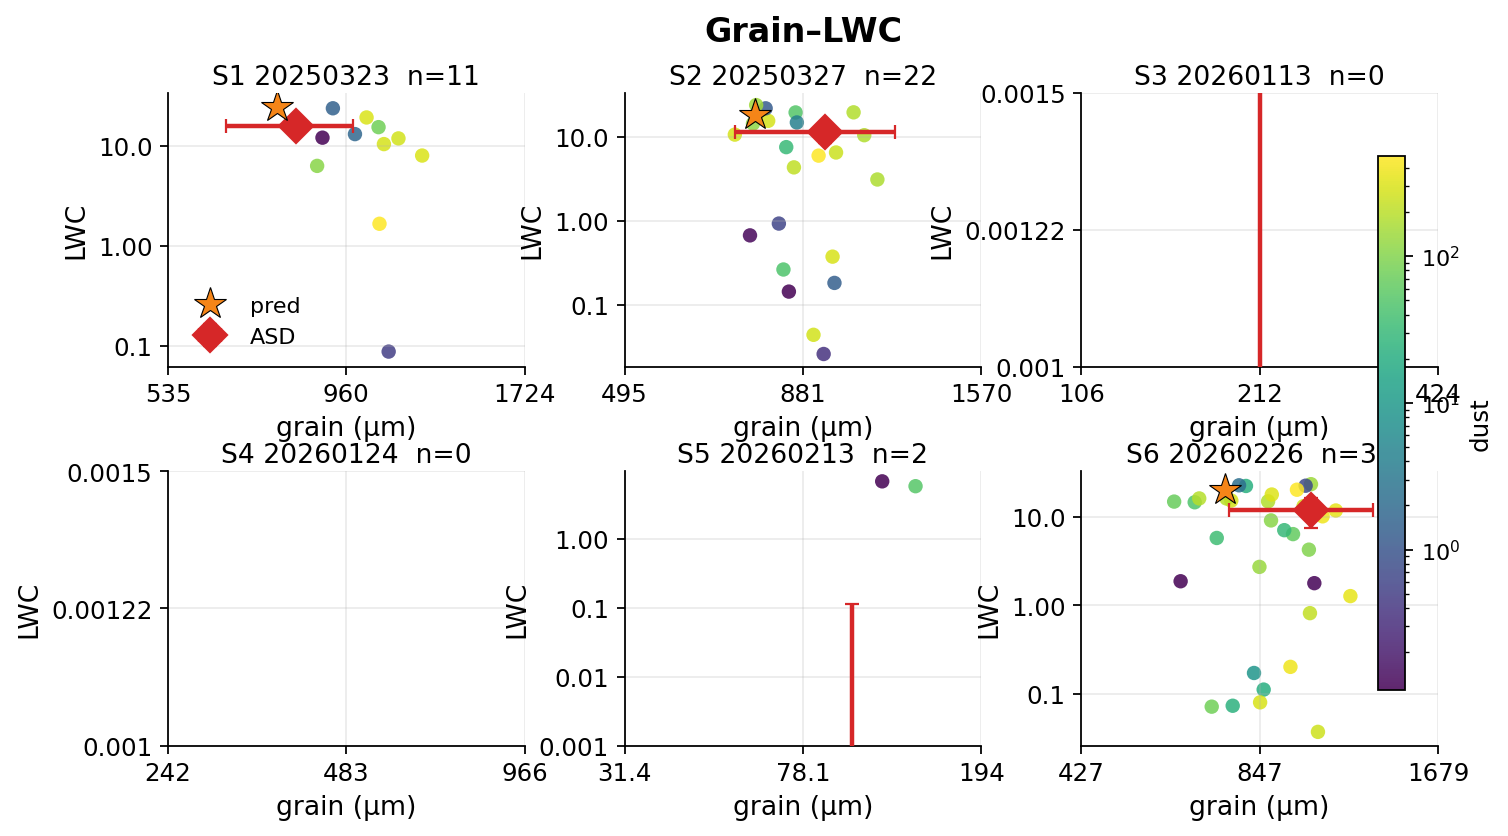
\includegraphics[width=\linewidth]{grain_lwc.png}
  \caption{grain vs.\ lwc}
\end{subfigure}

\vspace{0.6em}
\begin{subfigure}[t]{0.32\textwidth}
  \centering
  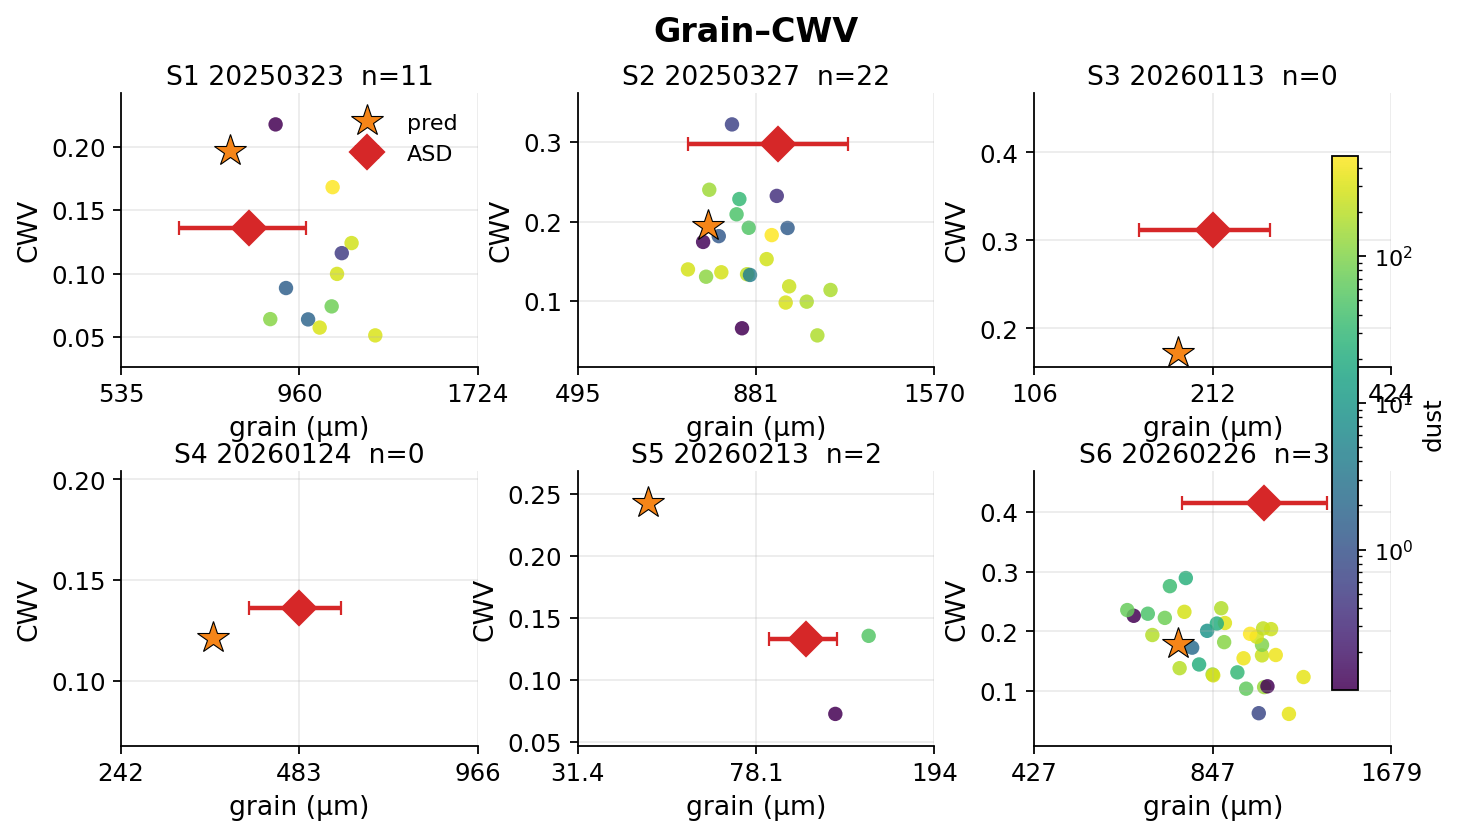
\includegraphics[width=\linewidth]{grain_cwv.png}
  \caption{grain vs.\ cwv}
\end{subfigure}\hspace{0.02\textwidth}
\begin{subfigure}[t]{0.32\textwidth}
  \centering
  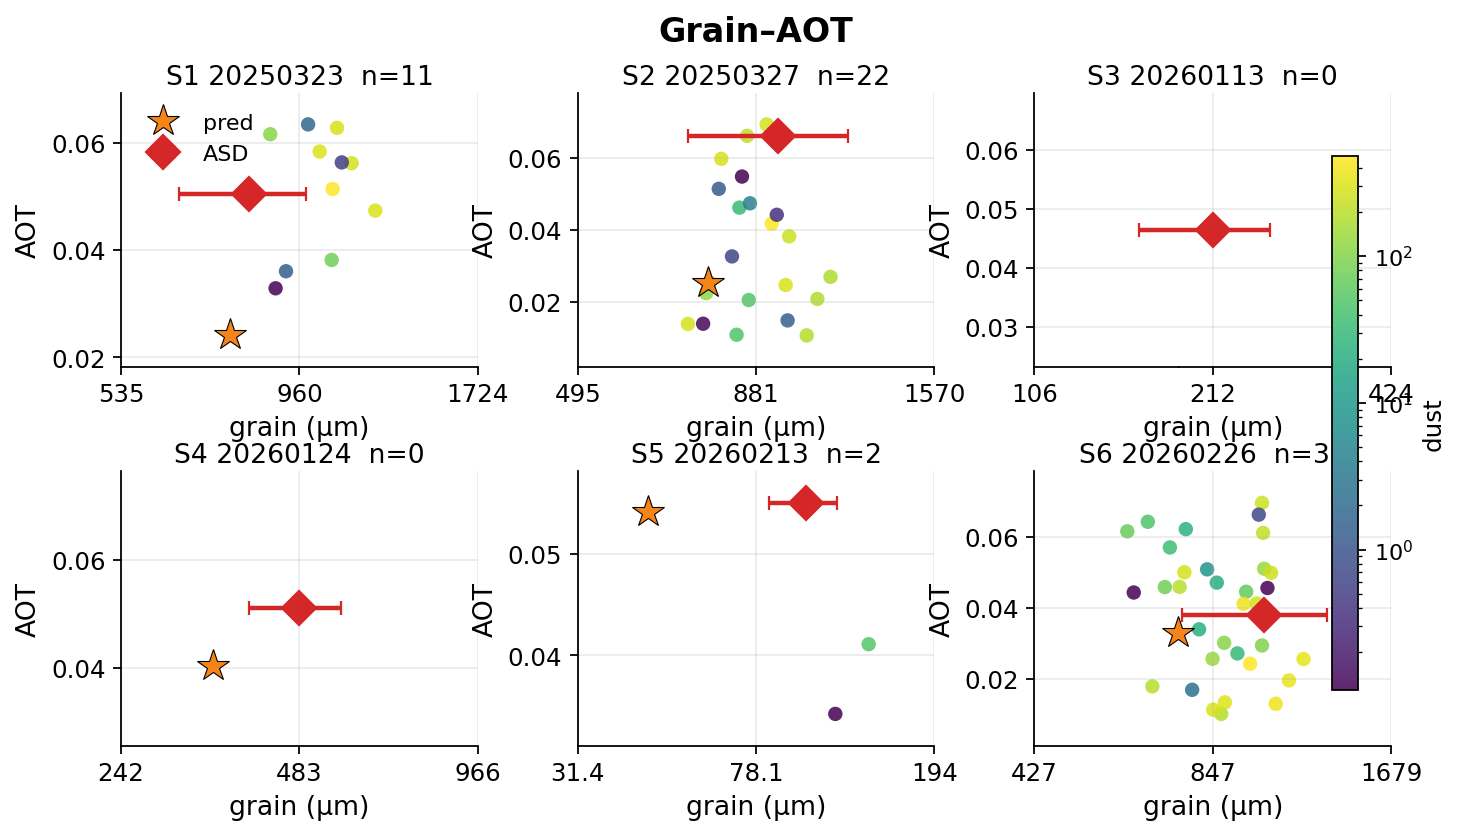
\includegraphics[width=\linewidth]{grain_aot.png}
  \caption{grain vs.\ aot}
\end{subfigure}
\caption{ASD grain-size pairs against other QoIs (compact diagnostics from the Sept.\ analysis).}
\label{fig:asd-grain-pairs}
\end{figure}

\FloatBarrier

%==============================================================================
\section{Discussion}
\label{sec:discussion}
%==============================================================================

Several conclusions follow from the combined interim and final experiments.

\begin{enumerate}[leftmargin=1.3em]
  \item \textbf{Problem conditioning dominates architecture.}
        Moving from unconstrained 11-QoI mixtures to pure-snow seven-QoI improved
        aggregate RRMSE by an order of magnitude before any final architecture bake-off.
        Surrogates cannot compensate for designs that wash out spectral signatures.
  \item \textbf{Physics-based simulation  accuracy does not imply field transfer.}
        TabPFN and PCA-GP lead on simulator test RRMSE/NIS, yet ASD aggregates remain
        large and coverage is miscalibrated.
        Closing the simulator--field gap (domain randomization, ASD-informed DOE,
        multi-fidelity calibration) is now as important as refining kernels.
  \item \textbf{NI-SORF Mat\'ern-$3/2$ is a strong kernel contender.}
        It matches or beats other SORF/SVGP variants on several physics-based simulation QoIs
        (especially $cos(i)$, grain size, and dust) while retaining GP-style
        uncertainty---a favorable profile when TabPFN-level inference cost is
        unacceptable.
  \item \textbf{Cost versus accuracy is application-dependent.}
        SVGP is the practical choice for rapid iteration and dense maps; SORF-MTGP buys
        joint structure at higher cost; TabPFN inverts the usual tradeoff.
  \item \textbf{Physical bounds remain open.}
        Soft warps alone do not keep predictive means inside design ranges; hard
        constraints or truncated predictives still need systematic study.
\end{enumerate}

%==============================================================================
\section{Conclusions and future work}
\label{sec:conclusion}
%==============================================================================

This project delivered scalable random-feature and variational GP emulators for
EMIT-like TOA radiance, grounded in GP$+$~\cite{yousefpour2024gpplus} and validated
against TabPFN and exact/partitioned GP baselines.
Mid-project experiments established reliable two-QoI baselines, diagnosed the failure
of unconstrained global 11-QoI emulation, and recovered strong pure-snow seven-QoI
performance (aggregate RRMSE $\approx0.05$).
Final Sept.\ results show that several models---especially TabPFN, PCA-GP, and
NI-SORF Mat\'ern-$3/2$---meet or approach the presentation accuracy targets on
physics-based simulation test data for geometry and grain-related QoIs, while algae/$aot$ and
ASD field transfer remain open challenges.

Priority next steps are:
(i)~ASD-aware dataset design with mixed-snow areal fractions (e.g., $fsnow$ in
$70\%$--$100\%$) rather than unconstrained Sobol' endmember logits;
(ii)~NIGP and lengthscale ablations on difficult QoIs;
(iii)~re-attempting broader multi-QoI emulation after those design and regularization
changes; and
(iv)~cost-aware model selection for operational mapping (SVGP or NI-SORF for speed,
heavier models for offline analysis).

\bibliographystyle{unsrtnat}
\bibliography{ref}

\end{document}
